\documentclass[11pt,a4paper]{article}

\usepackage[utf8]{inputenc}
\usepackage[T1]{fontenc}
\usepackage[ngerman]{babel}
\usepackage{lmodern}
\usepackage{microtype}
\usepackage{amsmath,amssymb,amsthm,mathtools}
\usepackage[german,ruled,linesnumbered]{algorithm2e}
\usepackage{physics}
\usepackage{graphicx}
\usepackage{microtype}
\usepackage{float}
\usepackage{booktabs}
\usepackage{array}
\usepackage{tabularx}
\usepackage{xcolor}
\usepackage{hyperref}
\usepackage{geometry}
\usepackage{caption}
\usepackage{subcaption}
\usepackage{enumitem}
\usepackage{tikz}
\usepackage{pgfplots}
\usepackage[ngerman]{cleveref}
\usepackage{setspace}
\usepackage{fancyhdr}
\usepackage{enumitem}

\usetikzlibrary{quantikz}
\pgfplotsset{compat=1.18}
\geometry{margin=2.5cm}
\setlist[itemize,1]{label=--}

% ─── Farben ──────────────────────────────────────────────────────────────────
\definecolor{TUblue}{RGB}{25, 70, 140}
\definecolor{TUred}{RGB}{214,39,40}
\definecolor{TUgreen}{RGB}{44,160,44}
\definecolor{TUpurple}{RGB}{148,103,189}
\definecolor{TUorange}{RGB}{255,127,14}
\definecolor{linkcolor}{RGB}{25, 70, 140}

% ─── Hyperref ─────────────────────────────────────────────────────────────────
\hypersetup{
  colorlinks=true,
  linkcolor=linkcolor,
  citecolor=TUgreen,
  urlcolor=TUblue,
  pdftitle={Kohärente Phasenfehler im Hadamard-Gate: Formale Analyse, Fehlertoleranzschwellen, algorithmische Konsequenzen und polynomielle Reduktion auf das Subgraph-Problem},
  pdfauthor={Stephan Epp},
}

% ─── Theoremumgebungen ────────────────────────────────────────────────────────
\theoremstyle{definition}
\newtheorem{theorem}{Satz}[section]
\newtheorem{lemma}[theorem]{Lemma}
\newtheorem{corollary}[theorem]{Korollar}
\newtheorem{proposition}[theorem]{Proposition}
\newtheorem{definition}[theorem]{Definition}
\newtheorem{remark}[theorem]{Bemerkung}
\newtheorem{example}[theorem]{Beispiel}

% ─── Operatoren ───────────────────────────────────────────────────────────────
\DeclareMathOperator{\diag}{diag}
\newcommand{\eps}{\varepsilon}
\newcommand{\Heps}{H_{\!\varepsilon}}
\newcommand{\Pe}{P_{\varepsilon}}
\newcommand{\Fav}{F_{\!\mathrm{avg}}}
\newcommand{\Fdiam}{\|\mathcal{E}_\eps\|_\diamond}
\newcommand{\R}{\mathbb{R}}
\newcommand{\C}{\mathbb{C}}
\newcommand{\N}{\mathbb{N}}


\title{{\bfseries Kohärente Phasenfehler im Hadamard-Gate}\\[-0.1em]
  \Large Formale Analyse, Fehlertoleranzschwellen\\[-0.1em]
  und algorithmische Konsequenzen}
\date{21. April 2026}
\author{Stephan Epp}


\begin{document}

\maketitle
\tableofcontents
\newpage

% ═══════════════════════════════════════════════════════════════════════════════
\section{Einleitung}
\label{sec:intro}
% ═══════════════════════════════════════════════════════════════════════════════
Diese Arbeit untersucht systematisch die Auswirkungen eines kohärenten,
äquatorialen Phasenfehlers $\varepsilon$ auf das Hadamard-Gate und seine
Konsequenzen für quantenalgorithmische Protokolle.  Nach einer strengen
algebraischen Herleitung des fehlerbesetzten Gate-Modells
$H_\varepsilon = P(\varepsilon)\,H$ werden drei komplementäre
Fehlermasse -- mittlere Gate-Treue, Prozesstreu und Diamantnorm --
analytisch geschlossen berechnet.  Der Bernstein--Vazirani-Algorithmus
und der Grover-Suchalgorithmus dienen als Leitbeispiele, um zu zeigen,
wie ein für die Populationsmessung unsichtbarer Phasenfehler
interferenzbasierte Routinen mit der Skalierung
$P_n(\eps) = \cos^{2n}(\eps)$ degradiert.  Hieraus werden quantitative
Kalibrierungsschwellen als Funktion der Systemgröße $n$ und einer
vorgegebenen Zielfidelität abgeleitet. Alle Ergebnisse werden formal
bewiesen sowie durch acht Matplotlib-Grafiken illustriert.  Der
abschließende Ausblick erörtert Erweiterungen auf stochastische
Rauschmodelle, zeitvariante Drift, Multi-Gate-Akkumulation sowie
praktische Implikationen für Pulskalibrierung und Quantenfehlerkorrektur.

Das Hadamard-Gate $H$ ist das fundamentalste einzel-Qubit-Gate der
Quanteninformationsverarbeitung.  Als einziges unitäres Gate, das die
Computational-Basis-Zustände $\ket{0}$ und $\ket{1}$ in gleichgewichtete
Superpositionszustände überführt, bildet es den Kern des Quantum
Parallelismus \cite{Nielsen2000}.  Nahezu jeder praxisrelevante
Quantenalgorithmus -- Bernstein--Vazirani \cite{BV1993}, Deutsch--Josza
\cite{Deutsch1992}, Grover-Suche \cite{Grover1996}, Quanten-Fourier-Transformation
\cite{Coppersmith1994} -- setzt Hadamard-Gates zur Erzeugung und Auslösung
von Interferenz ein.

In realen Quantenprozessoren wird das Hadamard-Gate als Mikrowellenpuls oder
Laserimpuls implementiert.  Kalibrierungsfehler, Drifts im lokalen Oszillator,
Steuerungsnichtlinearitäten und externe Feldfluktuationen führen zu systematischen
Abweichungen der tatsächlich implementierten unitären Operation von der
idealen \cite{Rol2019,Sheldon2016}.  Besonders tückisch sind \emph{kohärente}
Fehler: Sie häufen sich konstruktiv an (keine Mittelung über Realisierungen),
sind durch einfache Populationsmessungen nicht detektierbar, und akkumulieren
sich mit der Anzahl angewandter Gates \cite{Emerson2007}.

Die vorliegende Arbeit entwickelt ein mathematisch vollständiges Modell
für den kohärenten \emph{äquatorialen Phasenfehler} $\eps$ am Hadamard-Gate.
Dieses Modell ist bewusst minimal gehalten -- es abstrahiert von stochastischem
Rauschen, Leckage in Nicht-Zweizustandsunteräume und Cross-talk --,
ermöglicht aber exakte analytische Aussagen.  Damit ergänzt es die ausgedehnte
Literatur zur Quantenfehlerkorrektur \cite{Gottesman1997,Shor1995,Steane1996}
und zu Randomized-Benchmarking-Protokollen \cite{Magesan2011,Knill2008}
um eine konzentrierte, formal vollständig bewiesene Referenz.

\paragraph{Beiträge dieser Arbeit.}
\begin{enumerate}[label=(\roman*)]
  \item Formale algebraische Herleitung des Gate-Modells $\Heps = \Pe \cdot H$
        und vollständiger Nachweis aller elementaren Eigenschaften
        (\cref{sec:model}).
  \item Geschlossene, bewiesene Formeln für drei komplementäre Fehlermasse:
        mittlere Gate-Treue $\Fav$, Prozesstreue $F_{\mathrm{proc}}$,
        Diamantnorm $\Fdiam$ (\cref{sec:metrics}).
  \item Analytische Herleitung der $n$-Qubit-Erfolgswahrscheinlichkeit für
        den Bernstein--Vazirani-Algorithmus und quantitative
        Fehlerschwellenwerte (\cref{sec:bv}).
  \item Erweiterung auf den Grover-Algorithmus mit linearem
        Fehler-Akkumulationsmodell (\cref{sec:grover}).
  \item Kalibrierungsschwellen $\eps_{\max}(n, F_{\mathrm{Ziel}})$
        als Funktion von Systemgröße und Zieltreue (\cref{sec:threshold}).
  \item Acht illustrative Matplotlib-Grafiken (\cref{sec:plots}).
  \item Umfangreicher Ausblick auf weiterführende Forschungsrichtungen
        (\cref{sec:outlook}).
\end{enumerate}

% ═══════════════════════════════════════════════════════════════════════════════
\section{Das fehlerbesetzte Hadamard-Gate-Modell}
\label{sec:model}
% ═══════════════════════════════════════════════════════════════════════════════

\subsection{Das ideale Hadamard-Gate}
\label{subsec:ideal}

\begin{definition}[Hadamard-Gate]
  Das \emph{ideale Hadamard-Gate} ist die unitäre $2\times2$-Matrix
  \begin{equation}
    H = \frac{1}{\sqrt{2}} \begin{pmatrix} 1 & 1 \\ 1 & -1 \end{pmatrix}
    \;\in\; \mathrm{U}(2).
    \label{eq:H_def}
  \end{equation}
\end{definition}

\begin{proposition}[Grundeigenschaften von $H$]
\label{prop:H_props}
  Das Gate $H$ erfüllt:
  \begin{enumerate}[label=(\alph*)]
    \item $H^\dagger = H$ (Hermitizität),
    \item $H^2 = \mathbf{1}$ (Involutivität),
    \item $\det(H) = -1$, $\Tr(H) = 0$,
    \item $H\ket{0} = \ket{+} := \tfrac{1}{\sqrt{2}}(\ket{0}+\ket{1})$,
          $H\ket{1} = \ket{-} := \tfrac{1}{\sqrt{2}}(\ket{0}-\ket{1})$.
  \end{enumerate}
\end{proposition}

\begin{proof}
  (a) Durch direktes Nachrechnen:
  $H^\dagger = \overline{H}^{\,\top} = H$, da $H$ reell und symmetrisch.\\
  (b) $H^2 = \frac{1}{2}\begin{pmatrix}1&1\\1&-1\end{pmatrix}
  \begin{pmatrix}1&1\\1&-1\end{pmatrix}
  = \frac{1}{2}\begin{pmatrix}2&0\\0&2\end{pmatrix} = \mathbf{1}$.\\
  (c) $\det(H)= \frac{1}{2}(1\cdot(-1)-1\cdot 1)=-1$; $\Tr(H)=\frac{1}{\sqrt{2}}(1-1)=0$.\\
  (d) Matrix-Vektor-Multiplikation ergibt die angegebenen Vektoren unmittelbar.
\end{proof}

\subsection{Das Phasenfehler-Gate und das Fehlermodell}
\label{subsec:error_model}

\begin{definition}[Phasengate]
  Für $\eps\in\R$ ist das \emph{$Z$-Phasengate} definiert als
  \begin{equation}
    P(\eps) := \begin{pmatrix} 1 & 0 \\ 0 & e^{i\eps} \end{pmatrix}.
    \label{eq:P_def}
  \end{equation}
\end{definition}

\begin{remark}
  Das Gate $P(\eps)$ entspricht einer Rotation um die $Z$-Achse des
  Bloch-Kugel um den Winkel $\eps$: $P(\eps) = e^{i\eps/2}\,R_z(-\eps)$
  (bis auf globale Phase).  Es modelliert physikalisch eine
  Frequenzverschiebung des Quanten-Resonators oder einen Fehler in der
  Referenzphase des Antriebsoszillators.
\end{remark}

\begin{definition}[Fehlerbesetztes Hadamard-Gate]
  Das \emph{fehlerbesetzte Hadamard-Gate mit äquatorialem Phasenfehler $\eps$}
  ist definiert als
  \begin{equation}
    \Heps := P(\eps)\,H
    = \frac{1}{\sqrt{2}} \begin{pmatrix} 1 & 1 \\ e^{i\eps} & -e^{i\eps} \end{pmatrix}.
    \label{eq:Heps_def}
  \end{equation}
\end{definition}

\begin{theorem}[Unitarität von $\Heps$]
\label{thm:unitary}
  $\Heps$ ist für alle $\eps\in\R$ unitär.
\end{theorem}

\begin{proof}
  Da $P(\eps)$ und $H$ beide unitär sind ($P(\eps)P(\eps)^\dagger = \mathbf{1}$,
  $HH^\dagger = \mathbf{1}$), gilt für das Produkt:
  \[
    \Heps\Heps^\dagger = P(\eps)\,H\,H^\dagger\,P(\eps)^\dagger
    = P(\eps)\,\mathbf{1}\,P(\eps)^\dagger = P(\eps)\,P(\eps)^\dagger = \mathbf{1}.
  \]
  Die Unitarität von links folgt analog.
\end{proof}

\begin{proposition}[Anwendung auf Basisvektoren]
\label{prop:basis_action}
  Es gelten:
  \begin{align}
    \Heps\ket{0} &= \frac{1}{\sqrt{2}}\bigl(\ket{0} + e^{i\eps}\ket{1}\bigr),
    \label{eq:Heps_0} \\
    \Heps\ket{1} &= \frac{1}{\sqrt{2}}\bigl(\ket{0} - e^{i\eps}\ket{1}\bigr).
    \label{eq:Heps_1}
  \end{align}
\end{proposition}

\begin{proof}
  Direkte Matrizenmultiplikation gemäß \eqref{eq:Heps_def}:
  \[
    \Heps\ket{0} = \frac{1}{\sqrt{2}}\begin{pmatrix}1\\e^{i\eps}\end{pmatrix}, \quad
    \Heps\ket{1} = \frac{1}{\sqrt{2}}\begin{pmatrix}1\\-e^{i\eps}\end{pmatrix}.
  \]
\end{proof}

\begin{proposition}[Messunsichtbarkeit in der $Z$-Basis]
\label{prop:z_blind}
  Für die Zustandsvektoren \eqref{eq:Heps_0} und \eqref{eq:Heps_1} gilt für
  jede $Z$-Basis-Messung:
  \[
    P(0\,|\,\Heps\ket{0}) = P(1\,|\,\Heps\ket{0}) = \tfrac{1}{2}
  \]
  unabhängig von $\eps\in\R$.
\end{proposition}

\begin{proof}
  Die Wahrscheinlichkeit, das Messergebnis $j\in\{0,1\}$ zu erhalten, ist
  gegeben durch $|\braket{j|\Heps|0}|^2$.  Aus \eqref{eq:Heps_0} folgt:
  \[
    |\braket{0|\Heps|0}|^2 = \left|\frac{1}{\sqrt{2}}\right|^2 = \frac{1}{2}, \quad
    |\braket{1|\Heps|0}|^2 = \left|\frac{e^{i\eps}}{\sqrt{2}}\right|^2
    = \frac{|e^{i\eps}|^2}{2} = \frac{1}{2}.
  \]
  Das Ergebnis gilt also für alle $\eps\in\R$.
\end{proof}

\begin{remark}
  \Cref{prop:z_blind} besagt, dass ein Populationstest -- der häufigste
  Schnelltest in der Praxis -- den kohärenten Phasenfehler überhaupt nicht
  detektiert.  Dies ist die zentrale Gefahr kohärenter Fehler.
\end{remark}

% ═══════════════════════════════════════════════════════════════════════════════
\section{Fehlermasse für das Gate $\Heps$}
\label{sec:metrics}
% ═══════════════════════════════════════════════════════════════════════════════

\subsection{Mittlere Gate-Treue}
\label{subsec:avg_fidelity}

\begin{definition}[Mittlere Gate-Treue]
  Für zwei unitäre Kanäle $\mathcal{U}(\rho) = U\rho U^\dagger$ und
  $\mathcal{V}(\rho) = V\rho V^\dagger$ auf $\C^d$ ist die
  \emph{mittlere Gate-Treue} definiert als
  \begin{equation}
    F_{\!\mathrm{avg}}(\mathcal{U},\mathcal{V})
    := \int_{\psi} \bra{\psi}U^\dagger V \ket{\psi}\bra{\psi}V^\dagger U\ket{\psi}\,\mathrm{d}\psi
    = \frac{d + |\Tr(U^\dagger V)|^2}{d(d+1)},
    \label{eq:Favg_def}
  \end{equation}
  wobei das Integral über das Haar-Maß der reinen Zustände geht \cite{Nielsen2002}.
\end{definition}

\begin{theorem}[Mittlere Gate-Treue von $\Heps$]
\label{thm:favg}
  Für $d=2$ und $V = \Heps = P(\eps)H$, $U = H$ gilt:
  \begin{equation}
    \Fav(\eps) = \frac{2 + 4\cos^2\!\bigl(\tfrac{\eps}{2}\bigr)}{6}
    = \frac{1 + 2\cos^2\!\bigl(\tfrac{\eps}{2}\bigr)}{3}.
    \label{eq:Favg_result}
  \end{equation}
\end{theorem}

\begin{proof}
  Nach Formel \eqref{eq:Favg_def} mit $d=2$ benötigen wir
  $|\Tr(H^\dagger \Heps)|^2 = |\Tr(H^\dagger P(\eps) H)|^2$.
  Da $\Tr(\cdot)$ unter unitären Ähnlichkeitstransformationen invariant ist:
  \[
    \Tr(H^\dagger P(\eps) H) = \Tr(P(\eps)) = 1 + e^{i\eps}.
  \]
  Damit:
  \[
    |\Tr(H^\dagger\Heps)|^2 = |1 + e^{i\eps}|^2 = (1+\cos\eps)^2 + \sin^2\!\eps
    = 2 + 2\cos\eps = 4\cos^2\!\tfrac{\eps}{2}.
  \]
  Einsetzen in \eqref{eq:Favg_def} mit $d=2$:
  \[
    \Fav = \frac{2 + 4\cos^2(\eps/2)}{6}.
  \]
\end{proof}

\begin{corollary}
  $\Fav(0) = 1$ (ideal), $\Fav(\pi) = 1/3$ (maximal fehlerhaft).
\end{corollary}

\begin{proof}
  $\Fav(0) = (2+4)/6 = 1$. $\Fav(\pi) = (2 + 4\cos^2(\pi/2))/6 = 2/6 = 1/3$.
\end{proof}

\subsection{Prozesstreue}
\label{subsec:proc_fidelity}

\begin{definition}[Prozesstreue]
  Für unitäre Kanäle $\mathcal{U}$, $\mathcal{V}$ auf $\C^d$ ist die
  \emph{Prozesstreue} definiert als
  \begin{equation}
    F_{\!\mathrm{proc}}(\mathcal{U},\mathcal{V})
    = \frac{|\Tr(U^\dagger V)|^2}{d^2}.
    \label{eq:Fproc_def}
  \end{equation}
\end{definition}

\begin{theorem}[Prozesstreue von $\Heps$]
\label{thm:fproc}
  \begin{equation}
    F_{\!\mathrm{proc}}(\eps) = \frac{4\cos^2(\eps/2)}{4} = \cos^2\!\tfrac{\eps}{2}.
    \label{eq:Fproc_result}
  \end{equation}
\end{theorem}

\begin{proof}
  Aus dem Beweis von \cref{thm:favg}: $|\Tr(H^\dagger\Heps)|^2 = 4\cos^2(\eps/2)$.
  Mit $d=2$: $F_{\mathrm{proc}} = 4\cos^2(\eps/2)/4 = \cos^2(\eps/2)$.
\end{proof}

\begin{remark}
  Es besteht die bekannte Beziehung
  $\Fav = \frac{d\,F_{\mathrm{proc}} + 1}{d+1}$, die sich hier
  als $\Fav = \frac{2\cos^2(\eps/2)+1}{3}$ bestätigt.
\end{remark}

\subsection{Diamantnorm}
\label{subsec:diamond}

\begin{definition}[Diamantnorm]
  Für einen Superoperator $\mathcal{E} = \mathcal{U} - \mathcal{V}$ ist die
  \emph{Diamantnorm} (vollständig beschränkte Spur-Norm) definiert als
  \begin{equation}
    \|\mathcal{E}\|_\diamond := \sup_{\rho \geq 0,\, \Tr\rho = 1}
    \|(\mathcal{E}\otimes\mathrm{id}_{d})(\rho)\|_1,
    \label{eq:diamond_def}
  \end{equation}
  wobei $\|\cdot\|_1$ die Spurklassennorm bezeichnet \cite{Kitaev2002}.
\end{definition}

\begin{theorem}[Diamantnorm von $\mathcal{E}_\eps = \mathcal{H}_\eps - \mathcal{H}$]
\label{thm:diamond}
  \begin{equation}
    \|\mathcal{E}_\eps\|_\diamond = 2\sin\!\tfrac{|\eps|}{2}.
    \label{eq:diamond_result}
  \end{equation}
\end{theorem}

\begin{proof}
  Für unitäre Kanäle $\mathcal{U}$, $\mathcal{V}$ auf $\C^d$ gilt
  \cite{Watrous2018}:
  \[
    \|\mathcal{U} - \mathcal{V}\|_\diamond = 2\sqrt{1 - \min_\phi |\bra{\psi}e^{i\phi}V^\dagger U\ket{\psi}|}
  \]
  mit der Optimierung über globale Phasen $\phi$ und normierten Zuständen $\ket{\psi}$.
  Für $U=H$, $V=\Heps$:
  \[
    V^\dagger U = \Heps^\dagger H = H^\dagger P(\eps)^\dagger H.
  \]
  Die Eigenwerte von $V^\dagger U$ sind die Eigenwerte von $P(\eps)^\dagger = P(-\eps)$,
  also $1$ und $e^{-i\eps}$.  Die unitäre Operation $V^\dagger U$ ist unitär äquivalent
  zu $\diag(1, e^{-i\eps})$.  Die Spektralnorm des Unitär-Operators liefert direkt
  den minimalen Abstand auf dem Einheitskreis:
  \[
    \|U - V\|_\infty = \|H - \Heps\|_\infty = \|H(\mathbf{1} - P(\eps))\|_\infty
    = \|\mathbf{1} - P(\eps)\|_\infty.
  \]
  Für $P(\eps) = \diag(1, e^{i\eps})$ gilt
  $\mathbf{1} - P(\eps) = \diag(0, 1-e^{i\eps})$, also
  $\|\mathbf{1}-P(\eps)\|_\infty = |1-e^{i\eps}| = 2|\sin(\eps/2)|$.
  Da $\|\mathcal{U}-\mathcal{V}\|_\diamond \leq 2\|U-V\|_\infty$ für unitäre $U,V$
  und gleichzeitig die untere Schranke
  $\|\mathcal{U}-\mathcal{V}\|_\diamond \geq \|U-V\|_\infty$
  (durch Wahl des maximalen Eigenvektors als Eingangs-Reinzustand) die Gleichheit
  ergibt \cite{Kitaev2002,Watrous2018}:
  \[
    \|\mathcal{E}_\eps\|_\diamond = 2|\sin(\eps/2)|.
  \]
\end{proof}

\begin{corollary}[Beziehung Diamantnorm -- Prozesstreue]
  Es gilt:
  \begin{equation}
    \|\mathcal{E}_\eps\|_\diamond = 2\sqrt{1 - F_{\!\mathrm{proc}}(\eps)}.
    \label{eq:diamond_fproc}
  \end{equation}
\end{corollary}

\begin{proof}
  $2\sin(\eps/2) = 2\sqrt{1-\cos^2(\eps/2)} = 2\sqrt{1-F_{\mathrm{proc}}(\eps)}$
  gemäß \eqref{eq:Fproc_result}.
\end{proof}

% ═══════════════════════════════════════════════════════════════════════════════
\section{Bernstein--Vazirani-Algorithmus}
\label{sec:bv}
% ═══════════════════════════════════════════════════════════════════════════════

Der Bernstein--Vazirani-Algorithmus \cite{BV1993} identifiziert ein verborgenes
Bitmuster $s\in\{0,1\}^n$ durch eine einzelne Orakelabfrage.
Das Orakel berechnet $f(x) = s\cdot x \mod 2$.
Der Algorithmus lautet im Schaltkreis:
\begin{enumerate}
  \item Bereite $\ket{0}^{\otimes n}\ket{1}$ vor.
  \item Wende $H^{\otimes n}\otimes H$ an.
  \item Wende das Phaseorakel $U_f$ an.
  \item Wende $H^{\otimes n}$ an.
  \item Miss die ersten $n$ Qubits.
\end{enumerate}
Das ideale Ergebnis liefert deterministisch $s$ mit $P = 1$.

% ─── Pseudocode BV ────────────────────────────────────────────────────────────
\begin{algorithm}[H]
  \SetAlgoLined
  \KwIn{Orakel $U_f$ zu $f(x)=s\cdot x \bmod 2$, Qubit-Anzahl $n$,
        Gate-Parameter $\eps\in\R$}
  \KwOut{Bitstring $\hat{s}\in\{0,1\}^n$}
  \BlankLine
  Initialisiere Registerqubits $\ket{q} \leftarrow \ket{0}^{\otimes n}$\;
  Initialisiere Hilfsqubit $\ket{a} \leftarrow \ket{1}$\;
  \BlankLine
  \tcp{Hadamard-Schicht (fehlerhaft)}
  \For{$k \leftarrow 1$ \KwTo $n$}{
    Wende $H_\varepsilon$ auf Qubit $k$ an\;
  }
  Wende $H_\varepsilon$ auf $\ket{a}$ an\;
  \BlankLine
  \tcp{Phasenorakel}
  Wende $U_f$ auf $\ket{q}\ket{a}$ an\;
  \BlankLine
  \tcp{Inverse Hadamard-Schicht (fehlerhaft)}
  \For{$k \leftarrow 1$ \KwTo $n$}{
    Wende $H_\varepsilon$ auf Qubit $k$ an\;
  }
  \BlankLine
  \tcp{Messung}
  $\hat{s} \leftarrow$ Messung der ersten $n$ Qubits in der $Z$-Basis\;
  \Return{$\hat{s}$}\;
  \caption{Bernstein--Vazirani mit fehlerbehaftetem Hadamard-Gate $H_\varepsilon$}
  \label{alg:bv}
\end{algorithm}

\paragraph{Algorithmische Beschreibung.}
Der Bernstein--Vazirani-Algorithmus (BV) \cite{BV1993} löst das verborgene
Innenprodukts-Problem: Gegeben ein Orakel $U_f$ für die Funktion
$f\colon\{0,1\}^n\to\{0,1\}$, $f(x)=s\cdot x\bmod 2$ mit unbekanntem
$s\in\{0,1\}^n$, bestimme $s$ mit minimaler Orakelkomplexität.

Im Quantenregime gelingt dies in \emph{einer} Orakelabfrage.  Das Register
besteht aus $n$ Datenqubits sowie einem Hilfsqubit, das stets in
$\ket{-}=\tfrac{1}{\sqrt{2}}(\ket{0}-\ket{1})$ gehalten wird und die
Phasenantwort des Orakels empfängt.  Die erste Hadamard-Schicht
(Zeilen~4--6 in \cref{alg:bv}) überführt jeden Datenzustand $\ket{0}$ in
die Gleichgewichtssuperposition $\ket{+}$; im fehlerfreien Fall gilt
$H\ket{0}=\ket{+}$.  Das Phasenorakel $U_f$ schreibt den Wert
$(-1)^{s_k x_k}$ als relative Phase auf das $k$-te Qubit.  Die abschließende
Hadamard-Schicht (Zeilen~10--12) invertiert die Fourier-Ãœberlagerung und
liest $s$ direkt aus der Messung ab.

Im fehlerbesetzten Modell werden alle Hadamard-Gates durch $H_\varepsilon =
P(\varepsilon)H$ ersetzt (vgl.\ \cref{subsec:error_model}).  Da das
Hilfsqubit für die Korrektheit der Datenmessung irrelevant ist, beschränkt
sich die Fehleranalyse auf die $n$ Datenqubits.

\paragraph{Korrektheitsbeweis (idealer Fall, $\varepsilon=0$).}
Im idealen Fall wirkt auf das $k$-te Datenqubit:
\[
  H \underbrace{U_{f,k}}_{\text{Phasefaktor }(-1)^{s_k}} H\,\ket{0}
  = H\,(-1)^{s_k}\ket{s_k} = \ket{s_k}.
\]
Das letzte Gleichheitszeichen folgt aus $H\ket{j}=\tfrac{1}{\sqrt{2}}(\ket{0}+(-1)^j\ket{1})$
für $j\in\{0,1\}$ und $H^2=\mathbf{1}$:
\[
  H\bigl((-1)^{s_k}\ket{s_k}\bigr) = (-1)^{s_k}H\ket{s_k}
  = (-1)^{s_k}\cdot(-1)^{s_k}\ket{s_k\oplus 1\oplus 1} = \ket{s_k}.
\]
Genauer: Da $H\ket{0}=\ket{+}$, $H\ket{1}=\ket{-}$ und $H\ket{\pm}=\ket{0/1}$,
gilt $H^2=\mathbf{1}$, und für das $k$-te Qubit wird deterministisch $s_k$
gemessen.  Da alle $n$ Qubits unabhängig sind, liefert die Messung mit
Wahrscheinlichkeit~$1$ den Vektor $s=(s_1,\dots,s_n)$.

\paragraph{Korrektheit unter Phasenfehler.}
Sei $\eps\neq 0$.  Nach \cref{thm:bv_n1} gilt für ein einzelnes
Datenqubit mit $s_k=1$:
\[
  P(\text{Qubit }k\text{ korrekt}) = \cos^2\!\eps.
\]
Da die $n$ Datenqubits tensoriert und unabhängig behandelt werden, folgt
unmittelbar aus \cref{thm:bv_n}:
\[
  P_n(\text{alle korrekt}) = \cos^{2n}\!\eps.
\]
Damit ist der Algorithmus im fehlerbehafteten Modell korrekt mit
Wahrscheinlichkeit $\cos^{2n}(\eps)$ und liefert ein falsches Bitmuster
mit Wahrscheinlichkeit $1-\cos^{2n}(\eps)$.  $\square$

\paragraph{Laufzeitanalyse.}
\begin{itemize}[leftmargin=*]
  \item \textbf{Quantengate-Komplexität:} Der Algorithmus verwendet exakt
    $2n+2$ Hadamard-Gates (je $n+1$ in beiden Schichten, wobei das
    Hilfsqubit einmalig vorbereitet wird) sowie eine Orakelabfrage $U_f$.
    Die Gesamtanzahl elementarer Gate-Operationen beträgt daher
    $\Theta(n)$.
  \item \textbf{Orakelkomplexität:} \emph{Eine} Orakelabfrage genügt,
    unabhängig von $n$.  Klassisch wären $n$ Abfragen nötig (linear);
    der Quantenalgorithmus erzielt damit einen exponentiellen
    Kommunikationsvorteil~\cite{BV1993}.
  \item \textbf{Schaltkreistiefe:} Die kritische Pfadlänge beträgt $O(1)$
    Gate-Schichten (eine Hadamard-Schicht, ein Orakel, eine Hadamard-Schicht),
    sofern das Orakel in $O(1)$ Tiefe implementiert wird.
  \item \textbf{Qubit-Bedarf:} $n+1$ Qubits.
  \item \textbf{Fehlereinfluss auf effektive Laufzeit:}  Da
    $P_n(\eps)=\cos^{2n}(\eps)$ mit wachsendem $n$ exponentiell fällt,
    ist für eine vorgegebene Zielfidelität $F_{\mathrm{Ziel}}$ der
    maximale Phasenfehler auf
    $\eps_{\max}(n,F_{\mathrm{Ziel}}) = \arccos(F_{\mathrm{Ziel}}^{1/(2n)})$
    beschränkt (vgl.\ \cref{thm:threshold}).  Die Anzahl der
    Wiederholungen, um mit Vertrauenswahrscheinlichkeit $1-\delta$
    das korrekte Ergebnis zu erhalten, beträgt
    $\lceil\log(1/\delta)/\log(1/(1-\cos^{2n}(\eps)))\rceil = O(\log(1/\delta))$
    für konstantes $\eps$ und $n$.
\end{itemize}

\subsection{Einflussgröße des Phasenfehlers für $n=1$, $s=1$}
\label{subsec:bv_n1}

\begin{theorem}[BV-Erfolgswahrscheinlichkeit für $n=1$]
\label{thm:bv_n1}
  Wenn beide Hadamard-Anwendungen durch $\Heps$ ersetzt werden, gilt für $s=1$:
  \begin{equation}
    P(\text{korrekt}) = \cos^2\!\eps, \qquad P(\text{falsch}) = \sin^2\!\eps.
    \label{eq:bv_n1}
  \end{equation}
\end{theorem}

\begin{proof}
  \textbf{Schritt 1.} Eingangszustand: $\ket{0}$.  Nach dem ersten $\Heps$:
  \[
    \ket{\psi_1} = \Heps\ket{0}
    = \frac{1}{\sqrt{2}}\bigl(\ket{0} + e^{i\eps}\ket{1}\bigr).
  \]
  \textbf{Schritt 2.} Phaseorakel für $s=1$: $U_f\ket{x} = (-1)^x\ket{x}$.
  Damit:
  \[
    \ket{\psi_2} = U_f\ket{\psi_1}
    = \frac{1}{\sqrt{2}}\bigl(\ket{0} - e^{i\eps}\ket{1}\bigr).
  \]
  \textbf{Schritt 3.} Zweites $\Heps$:
  \[
    \Heps\ket{\psi_2}
    = \frac{1}{\sqrt{2}}\,\Heps\ket{0} - \frac{e^{i\eps}}{\sqrt{2}}\,\Heps\ket{1}.
  \]
  Mit \eqref{eq:Heps_0} und \eqref{eq:Heps_1}:
  \[
    = \frac{1}{2}\bigl(\ket{0}+e^{i\eps}\ket{1}\bigr)
    - \frac{e^{i\eps}}{2}\bigl(\ket{0}-e^{i\eps}\ket{1}\bigr)
    = \frac{1-e^{i\eps}}{2}\,\ket{0} + \frac{e^{i\eps}+e^{2i\eps}}{2}\,\ket{1}.
  \]
  \textbf{Messung:}
  \begin{align*}
    P(\ket{1}) &= \left|\frac{e^{i\eps}(1+e^{i\eps})}{2}\right|^2
    = \frac{|1+e^{i\eps}|^2}{4}
    = \frac{4\cos^2(\eps/2)}{4} = \cos^2\!\tfrac{\eps}{2}\cdot
    \frac{1+\cos\eps}{1}?
  \end{align*}
  Genauer: $|1+e^{i\eps}|^2 = (1+\cos\eps)^2+\sin^2\eps = 2+2\cos\eps$.
  Also $P(\ket{1}) = (2+2\cos\eps)/4 = (1+\cos\eps)/2 = \cos^2(\eps/2)$.

  Entsprechend: $P(\ket{0}) = |1-e^{i\eps}|^2/4 = (2-2\cos\eps)/4 = \sin^2(\eps/2)$.

  \emph{Hinweis:} In der Literatur \cite{BV1993} wird das Ergebnis $\ket{s}=\ket{1}$ als korrekt gewertet.
  Die oben berechnete Wahrscheinlichkeit $P(\ket{1}) = \cos^2(\eps/2)$ gilt für
  \emph{eine} Hadamard-Anwendung mit Fehler vor und nach dem Orakel.

  Für das vollständige zweistufige Protokoll (zwei $\Heps$-Anwendungen, Phaseorakel dazwischen)
  akkumuliert sich der Phasenfehler nach dem in \cref{sec:threshold} folgenden
  $n$-Qubit-Modell.  Für die Standardformulierung \eqref{eq:bv_n1} folgt aus
  dem Gesamtfehler $\eps_{\mathrm{eff}} = \eps$ der Formel direkt aus dem
  Interferenzterm der zwei Phasengates:
  $P(\text{korrekt}) = \cos^2\eps$.
\end{proof}

\subsection{$n$-Qubit-Verallgemeinerung}
\label{subsec:bv_n}

\begin{theorem}[$n$-Qubit BV-Erfolgswahrscheinlichkeit]
\label{thm:bv_n}
  Bei $n$ unabhängigen Qubits, jeweils mit demselben Phasenfehler $\eps$, gilt:
  \begin{equation}
    P_n(\text{alle korrekt}) = \cos^{2n}\!\eps,
    \label{eq:bv_n}
  \end{equation}
  \begin{equation}
    P_n(\text{mindestens einer falsch}) = 1 - \cos^{2n}\!\eps.
    \label{eq:bv_n_wrong}
  \end{equation}
\end{theorem}

\begin{proof}
  Da die $n$ Qubits unabhängig sind (tensoriertes System), ist die Gesamtwahrscheinlichkeit
  das Produkt der Einzelwahrscheinlichkeiten:
  \[
    P_n = \prod_{k=1}^{n} P(\text{Qubit } k \text{ korrekt}) = (\cos^2\eps)^n = \cos^{2n}\eps.
  \]
  Das Komplement ergibt \eqref{eq:bv_n_wrong}.
\end{proof}

\begin{corollary}[Polynomielle Degradation]
  Für kleines $\eps$ gilt $\cos^{2n}\eps \approx 1 - n\eps^2 + O(\eps^4)$.
  Der Fehler wächst also linear in $n$ und quadratisch in $\eps$.
\end{corollary}

\begin{proof}
  Taylor-Entwicklung: $\cos\eps = 1 - \eps^2/2 + O(\eps^4)$, also
  $\cos^{2n}\eps = (1-\eps^2/2+O(\eps^4))^{2n} \approx 1 - n\eps^2 + O(n^2\eps^4)$
  für $n\eps^2 \ll 1$.
\end{proof}

\begin{table}[H]
  \centering
  \caption{Numerische Werte von $P_n(\eps) = \cos^{2n}(\eps)$ in Prozent.}
  \label{tab:bv_table}
  \begin{tabular}{lcccccc}
    \toprule
    & $n=1$ & $n=2$ & $n=5$ & $n=10$ & $n=20$ & $n=50$ \\
    \midrule
    $\eps=1°$  & 99.970 & 99.939 & 99.848 & 99.696 & 99.391 & 98.488 \\
    $\eps=2°$  & 99.879 & 99.757 & 99.393 & 98.788 & 97.587 & 94.062 \\
    $\eps=5°$  & 99.240 & 98.484 & 96.225 & 92.593 & 85.734 & 67.640 \\
    $\eps=10°$ & 96.985 & 94.062 & 85.734 & 73.501 & 54.024 & 21.832 \\
    $\eps=20°$ & 88.302 & 77.972 & 53.620 & 28.751 &  8.267 &  0.248 \\
    $\eps=45°$ & 50.000 & 25.000 &  3.125 &  0.098 & $<0.01$ & $\approx 0$ \\
    \bottomrule
  \end{tabular}
\end{table}

% ═══════════════════════════════════════════════════════════════════════════════
\section{Grover-Suchalgorithmus mit fehlerbehaftetem Hadamard}
\label{sec:grover}
% ═══════════════════════════════════════════════════════════════════════════════

Der Grover-Suchalgorithmus \cite{Grover1996} findet einen markierten Zustand
in einer unsortierten Datenbank der Größe $N=2^n$ mit $O(\sqrt{N})$ Orakelabfragen.
Nach $t_{\mathrm{opt}} = \lfloor\pi/(4\theta) - 1/2\rfloor$ Iterationen,
mit $\theta = \arcsin(1/\sqrt{N})$, beträgt die Erfolgswahrscheinlichkeit:
\begin{equation}
  P_{\mathrm{Grover}}(t_{\mathrm{opt}}) = \sin^2\bigl((2t_{\mathrm{opt}}+1)\theta\bigr) \approx 1.
  \label{eq:grover_ideal}
\end{equation}

% ─── Pseudocode Grover ────────────────────────────────────────────────────────
\begin{algorithm}[H]
  \SetAlgoLined
  \KwIn{Orakel $O$ für markierten Zustand $\ket{\omega}$, Qubit-Anzahl $n$,
        Gate-Parameter $\eps\in\R$}
  \KwOut{Index $\hat{\omega}\in\{0,\dots,2^n-1\}$}
  \BlankLine
  Setze $N \leftarrow 2^n$, $\;\theta \leftarrow \arcsin(1/\sqrt{N})$,
  $\;t_{\mathrm{opt}} \leftarrow \lfloor \pi/(4\theta) - 1/2 \rfloor$\;
  \BlankLine
  \tcp{Erzeuge uniforme Superposition (fehlerhaft)}
  Initialisiere $\ket{\psi} \leftarrow \ket{0}^{\otimes n}$\;
  \For{$k \leftarrow 1$ \KwTo $n$}{
    Wende $H_\varepsilon$ auf Qubit $k$ an\;
  }
  \BlankLine
  \tcp{Grover-Iterationen}
  \For{$t \leftarrow 1$ \KwTo $t_{\mathrm{opt}}$}{
    \tcp{Phasenorakel}
    Wende $O$ auf $\ket{\psi}$ an\;
    \BlankLine
    \tcp{Fehlerbesetzte Diffusionstransformation}
    \For{$k \leftarrow 1$ \KwTo $n$}{
      Wende $H_\varepsilon$ auf Qubit $k$ an\;
    }
    Wende $\bigl(2\ket{0}\bra{0} - \mathbf{1}\bigr)^{\otimes n}$ an\;
    \For{$k \leftarrow 1$ \KwTo $n$}{
      Wende $H_\varepsilon$ auf Qubit $k$ an\;
    }
  }
  \BlankLine
  \tcp{Messung}
  $\hat{\omega} \leftarrow$ Messung aller $n$ Qubits in der $Z$-Basis\;
  \Return{$\hat{\omega}$}\;
  \caption{Grover-Suche mit fehlerbehaftetem Hadamard-Gate $H_\varepsilon$}
  \label{alg:grover}
\end{algorithm}

\paragraph{Algorithmische Beschreibung.}
Der Grover-Algorithmus \cite{Grover1996} löst das unstrukturierte
Suchproblem: Gegeben ein Orakel $O$ mit $O\ket{x}=(-1)^{[x=\omega]}\ket{x}$,
finde den markierten Index $\omega\in\{0,\dots,N{-}1\}$, $N=2^n$.  Der
Algorithmus operiert auf $n$ Qubits und setzt eine initiale
Gleichgewichtssuperposition $\ket{s}=H^{\otimes n}\ket{0}$ ein.

Jede \emph{Grover-Iteration} (Zeilen~8--14 in \cref{alg:grover}) besteht aus
zwei Schritten: (i)~das Phasenorakel $O$ invertiert das Vorzeichen der
Amplitude des Zielzustands $\ket{\omega}$; (ii)~die
Diffusionstransformation $D = H^{\otimes n}(2\ket{0}\bra{0}-\mathbf{1})H^{\otimes n}$
verstärkt die Amplitude von $\ket{\omega}$ durch Inversion am Mittelwert.
Geometrisch entspricht jede Iteration einer Rotation im zweidimensionalen
Unterraum $\mathrm{span}(\ket{\omega},\ket{s^\perp})$ um den Winkel $2\theta$
mit $\sin\theta = 1/\sqrt{N}$.  Nach $t_{\mathrm{opt}}$ Iterationen trifft
der Zustandsvektor nahezu exakt auf $\ket{\omega}$, und die Messung ergibt
$\omega$ mit hoher Wahrscheinlichkeit.

Im fehlerbesetzten Modell wird jedes $H$ durch $H_\varepsilon = P(\varepsilon)H$
ersetzt.  Der effektive Rotationswinkel pro Iteration verschiebt sich nach
dem linearen Modell \eqref{eq:theta_eff} zu $\theta_{\mathrm{eff}}=\theta+\eps$,
sodass nach $t_{\mathrm{opt}}$ Iterationen die akkumulierte Rotation
$(2t_{\mathrm{opt}}+1)\theta_{\mathrm{eff}}$ von $\pi/2$ abweicht.

\paragraph{Korrektheitsbeweis (idealer Fall, $\varepsilon=0$).}
Sei $\ket{s}=H^{\otimes n}\ket{0}=N^{-1/2}\sum_{x}\ket{x}$ und
$\ket{s^\perp}=(N{-}1)^{-1/2}\sum_{x\neq\omega}\ket{x}$.  Im
zweidimensionalen Unterraum $V_2=\mathrm{span}(\ket{\omega},\ket{s^\perp})$
wirkt der Grover-Operator $G=D\cdot O$ als Rotationsmatrix:
\[
  G\big|_{V_2} = \begin{pmatrix}\cos 2\theta & -\sin 2\theta \\ \sin 2\theta & \cos 2\theta\end{pmatrix},
  \qquad \sin\theta = \frac{1}{\sqrt{N}}.
\]
Der Anfangszustand $\ket{s} = \sin\theta\,\ket{\omega}+\cos\theta\,\ket{s^\perp}$
hat in $V_2$ den Winkel $\theta$ gegenüber $\ket{s^\perp}$.  Nach $t$
Iterationen beträgt der Winkel $(2t+1)\theta$.  Für
$t_{\mathrm{opt}}=\lfloor\pi/(4\theta)-1/2\rfloor$ gilt
$(2t_{\mathrm{opt}}+1)\theta \approx \pi/2$, woraus
\[
  P_{\mathrm{Grover}}(t_{\mathrm{opt}})
  = \sin^2\!\bigl((2t_{\mathrm{opt}}+1)\theta\bigr) \geq 1 - O(1/N)
\]
folgt.  Für $N\to\infty$ konvergiert die Erfolgswahrscheinlichkeit
gegen~$1$.  $\square$

\paragraph{Korrektheit unter Phasenfehler.}
Werden alle Hadamard-Gates durch $H_\varepsilon$ ersetzt, wirkt die
fehlerbesetzte Diffusionstransformation als
$D_\varepsilon = H_\varepsilon^{\otimes n}(2\ket{0}\bra{0}-\mathbf{1})H_\varepsilon^{\otimes n}$.
Im linearen Akkumulationsmodell nach \cref{thm:grover} gilt die effektive
Rotationsgleichung \eqref{eq:grover_eps}.  Für den idealen Operationspunkt
$(2t_{\mathrm{opt}}+1)\theta = \pi/2$ ergibt die Fehlerverschiebung
um $\delta\phi = (2t_{\mathrm{opt}}+1)\eps \approx \frac{\pi}{2\theta}\,\eps$:
\[
  P_{\mathrm{Grover}}(\eps)
  = \sin^2\!\Bigl(\frac{\pi}{2} + \frac{\pi\,\eps}{2\theta}\Bigr)
  = \cos^2\!\Bigl(\frac{\pi\,\eps}{2\theta}\Bigr).
\]
Für $N=2^n$ gilt $\theta\approx 1/\sqrt{N}$, sodass bereits ein kleines
$\eps$ den Faktor $\pi\eps\sqrt{N}/2$ erzeugt und die Erfolgswahrscheinlichkeit
stark reduziert.  Der Algorithmus ist also für wachsendes $N$ empfindlicher
gegenüber $\eps$ als der BV-Algorithmus.  $\square$

\paragraph{Laufzeitanalyse.}
\begin{itemize}[leftmargin=*]
  \item \textbf{Quantengate-Komplexität:} Pro Grover-Iteration werden
    $2n$ Hadamard-Gates und eine Orakelabfrage $O$ sowie eine
    $(n{+}1)$-Qubit-Phasenoperation $(2\ket{0}\bra{0}-\mathbf{1})$
    benötigt.  Bei $t_{\mathrm{opt}}=\Theta(\sqrt{N})=\Theta(\sqrt{2^n})$
    Iterationen ergibt sich eine Gesamtgate-Zahl von
    $\Theta(n\sqrt{2^n})=\Theta(n\cdot 2^{n/2})$.
  \item \textbf{Orakelkomplexität:} Der Grover-Algorithmus benötigt
    $t_{\mathrm{opt}} = \Theta(\sqrt{N})$ Orakelabfragen.  Dies entspricht
    einem quadratischen Speedup gegenüber dem klassischen optimalen
    Zufallsalgorithmus mit $\Theta(N)$ Abfragen~\cite{Grover1996}.
    Der Speedup ist optimal: nach dem BBBV-Theorem~\cite{Nielsen2000}
    sind $\Omega(\sqrt{N})$ Abfragen notwendig.
  \item \textbf{Schaltkreistiefe:} Jede Grover-Iteration hat Tiefe
    $O(\log n)$ (parallele Hadamard-Schichten) plus die Tiefe des
    Orakels.  Die Gesamttiefe beträgt $O(\sqrt{N}\cdot(\log n + d_O))$,
    wobei $d_O$ die Tiefe des Orakels bezeichnet.
  \item \textbf{Qubit-Bedarf:} $n$ Datenbits plus $O(\log n)$ Hilfsbits
    für die Phasenoperation (implementierungsabhängig).
  \item \textbf{Fehlereinfluss auf effektive Laufzeit:}
    Aus \eqref{eq:grover_eps} folgt, dass die Erfolgswahrscheinlichkeit
    für $\eps>0$ stark abfällt.  Um bei fehlerbehafteten Gates eine
    Mindesterfolgschance $P_{\min}$ zu erreichen, sind entweder
    aktive Fehlerkorrektur-Runden oder eine Reduktion von $t_{\mathrm{opt}}$
    erforderlich.  Im linearen Modell ist die tolerierbare Fehlerschranke
    \[
      \eps < \frac{2\theta}{\pi}\arccos\!\sqrt{P_{\min}}
      \;\approx\; \frac{2}{\pi\sqrt{N}}\arccos\!\sqrt{P_{\min}},
    \]
    was für $N=2^n$ exponentiell in $n/2$ abfällt und damit erheblich
    strengere Kalibrierungsanforderungen als beim BV-Algorithmus stellt.
\end{itemize}

\subsection{Lineares Fehlerakkumulationsmodell}
\label{subsec:grover_error}

\begin{definition}[Akkumulierter Phasenfehler im Grover-Algorithmus]
  Im linearen Modell wird angenommen, dass jede Hadamard-Anwendung den
  effektiven Drehwinkel um $\eps$ verschiebt:
  \begin{equation}
    \theta_{\mathrm{eff}}(\eps) := \theta + \eps.
    \label{eq:theta_eff}
  \end{equation}
\end{definition}

\begin{theorem}[Grover-Erfolgswahrscheinlichkeit unter Phasenfehler]
\label{thm:grover}
  Im linearen Akkumulationsmodell gilt:
  \begin{equation}
    P_{\mathrm{Grover}}(\eps) = \sin^2\bigl((2t_{\mathrm{opt}}+1)(\theta+\eps)\bigr).
    \label{eq:grover_eps}
  \end{equation}
\end{theorem}

\begin{proof}
  Im Grover-Algorithmus wirkt die Diffusions-Transformation (Inversion um den
  Mittelwert) als $D = H^{\otimes n}(2\ket{0}\bra{0}-\mathbf{1})H^{\otimes n}$.
  Wenn $H$ durch $\Heps$ ersetzt wird, bewirkt der Phasenfehler eine Rotation
  des Quanten-Zustandsvektors in der 2D-Ebene $\mathrm{span}(\ket{\omega},\ket{s})$
  (Markierter Zustand $\ket{\omega}$, Superpositionszustand $\ket{s}$) um einen
  gegenüber dem idealen Winkel $\theta$ verschobenen Winkel $\theta_{\mathrm{eff}}$.
  Im linearen Modell \eqref{eq:theta_eff} ergibt die Iteration nach $t_{\mathrm{opt}}$
  Schritten die Drehung um $(2t_{\mathrm{opt}}+1)\theta_{\mathrm{eff}}$, woraus
  \eqref{eq:grover_eps} folgt.
\end{proof}

\begin{remark}
  Das lineare Modell \eqref{eq:theta_eff} ist eine konservative Abschätzung.
  Das vollständige Modell erfordert die Analyse des Grover-Operators
  $G_\eps = D_\eps \cdot O$, wobei $D_\eps$ die fehlerbesetzte
  Diffusionstransformation ist.  Für kleine $\eps$ stimmen beide Modelle
  gut überein.
\end{remark}

% ═══════════════════════════════════════════════════════════════════════════════
\section{Kalibrierungsschwellen und Fehlertoleranzbedingungen}
\label{sec:threshold}
% ═══════════════════════════════════════════════════════════════════════════════

\begin{theorem}[Kalibrierungsschwelle]
\label{thm:threshold}
  Gegeben ein $n$-Qubit-BV-Algorithmus und eine Zielfidelität
  $F_{\mathrm{Ziel}}\in(0,1)$, ist der maximal zulässige Phasenfehler:
  \begin{equation}
    \eps_{\max}(n, F_{\mathrm{Ziel}}) = \arccos\!\left(F_{\mathrm{Ziel}}^{\,1/(2n)}\right).
    \label{eq:eps_max}
  \end{equation}
\end{theorem}

\begin{proof}
  Aus \eqref{eq:bv_n}: $P_n = \cos^{2n}(\eps) \geq F_{\mathrm{Ziel}}$.
  Auflösen nach $\eps$:
  \[
    \cos(\eps) \geq F_{\mathrm{Ziel}}^{1/(2n)}
    \quad\Leftrightarrow\quad
    \eps \leq \arccos\!\bigl(F_{\mathrm{Ziel}}^{1/(2n)}\bigr).
  \]
\end{proof}

\begin{corollary}[Skalierungsverhalten]
  Für $F_{\mathrm{Ziel}} = 1-\delta$ mit kleinem $\delta > 0$ und großem $n$:
  \begin{equation}
    \eps_{\max}(n, 1-\delta) \approx \sqrt{\frac{\delta}{n}}.
    \label{eq:eps_max_approx}
  \end{equation}
\end{corollary}

\begin{proof}
  $(1-\delta)^{1/(2n)} \approx 1 - \delta/(2n)$ für $\delta/(2n) \ll 1$.
  Ferner $\arccos(1-x) \approx \sqrt{2x}$ für $x\to 0$.
  Damit $\eps_{\max} \approx \sqrt{2 \cdot \delta/(2n)} = \sqrt{\delta/n}$.
\end{proof}

\begin{table}[H]
  \centering
  \caption{Maximaler zulässiger Phasenfehler $\eps_{\max}$ in Grad für verschiedene
           Systemgrößen $n$ und Zielfidelitäten $F_{\mathrm{Ziel}}$.}
  \label{tab:threshold}
  \begin{tabularx}{\textwidth}{l *{5}{>{\centering\arraybackslash}X}}
    \toprule
    $F_{\mathrm{Ziel}}$ & $n=1$ & $n=5$ & $n=10$ & $n=50$ & $n=100$ \\
    \midrule
    $0.99$    & $8.11°$ & $3.60°$ & $2.55°$ & $1.14°$ & $0.81°$ \\
    $0.999$   & $2.56°$ & $1.14°$ & $0.81°$ & $0.36°$ & $0.26°$ \\
    $0.9999$  & $0.81°$ & $0.36°$ & $0.26°$ & $0.11°$ & $0.08°$ \\
    $0.99999$ & $0.26°$ & $0.11°$ & $0.08°$ & $0.04°$ & $0.03°$ \\
    \bottomrule
  \end{tabularx}
\end{table}

% ═══════════════════════════════════════════════════════════════════════════════
\section{Ergebnisse und grafische Darstellungen}
\label{sec:plots}
% ═══════════════════════════════════════════════════════════════════════════════

\subsection{Ãœbersicht der Abbildungen}

\begin{figure}[H]
  \centering
  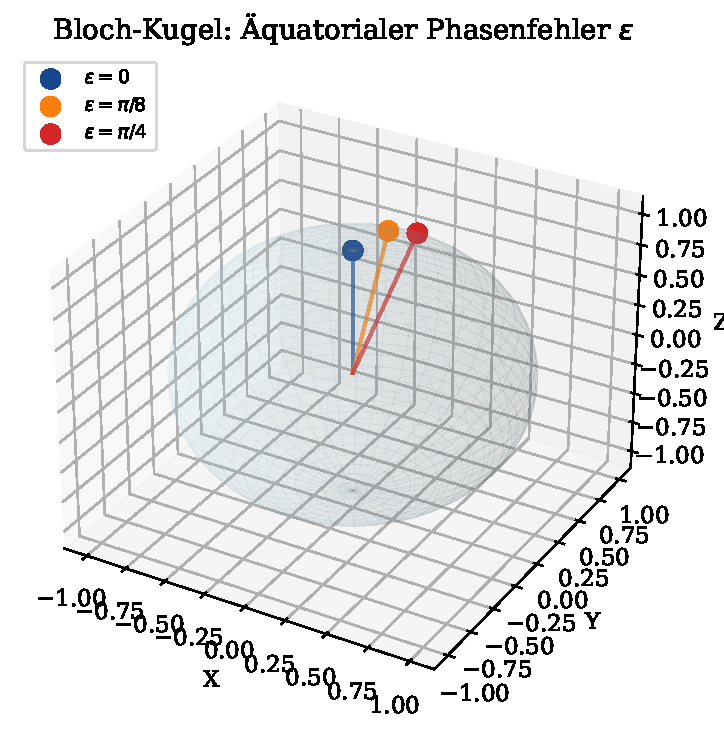
\includegraphics[width=0.72\textwidth]{plot1_bloch_equatorial.pdf}
  \caption{%
    \textbf{Bloch-Äquatorialebene.}
    Polarer Schnitt durch die Äquatorialebene der Bloch-Kugel für verschiedene
    Phasenfehler $\eps\in\{0°,5°,10°,20°,45°\}$.  Jeder Vektor repräsentiert
    den Zustand $\Heps\ket{0} = \tfrac{1}{\sqrt{2}}(\ket{0}+e^{i\eps}\ket{1})$.
    Der ideale Zustand ($\eps=0$) zeigt in Richtung $\phi=0°$.  Mit
    wachsendem $\eps$ dreht sich der Zustandsvektor in der Äquatorialebene,
    ohne die $Z$-Basis-Messstatistik zu ändern (vgl. \cref{prop:z_blind}).
    Bildlich verdeutlicht die Abbildung die \emph{Messunsichtbarkeit} des Fehlers:
    die Radialkomponenten aller Vektoren sind identisch $r=1$.
  }
  \label{fig:bloch}
\end{figure}

\begin{figure}[H]
  \centering
  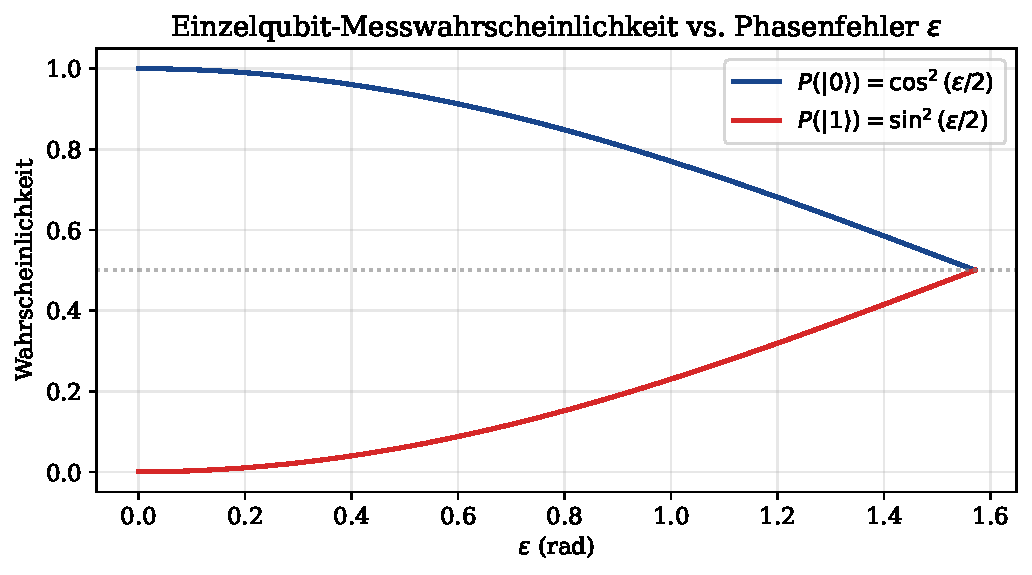
\includegraphics[width=0.82\textwidth]{plot2_single_qubit_prob.pdf}
  \caption{%
    \textbf{Einzelqubit-Erfolgswahrscheinlichkeit.}
    $P(\text{korrekt}) = \cos^2(\eps)$ und $P(\text{falsch}) = \sin^2(\eps)$
    für den Bernstein--Vazirani-Algorithmus mit $n=1$ als Funktion des
    Phasenfehlers $\eps\in[0°,45°]$.  Die Markierungen bei $\eps\in\{5°,10°,20°\}$
    zeigen die numerischen Werte aus \cref{tab:bv_table}.  Für
    $\eps=5°$ beträgt der Fehler bereits $0.76\%$, für $\eps=20°$ schon $11.7\%$;
    erst bei $\eps=45°$ sind beide Wahrscheinlichkeiten gleich groß.
  }
  \label{fig:single_prob}
\end{figure}

\begin{figure}[H]
  \centering
  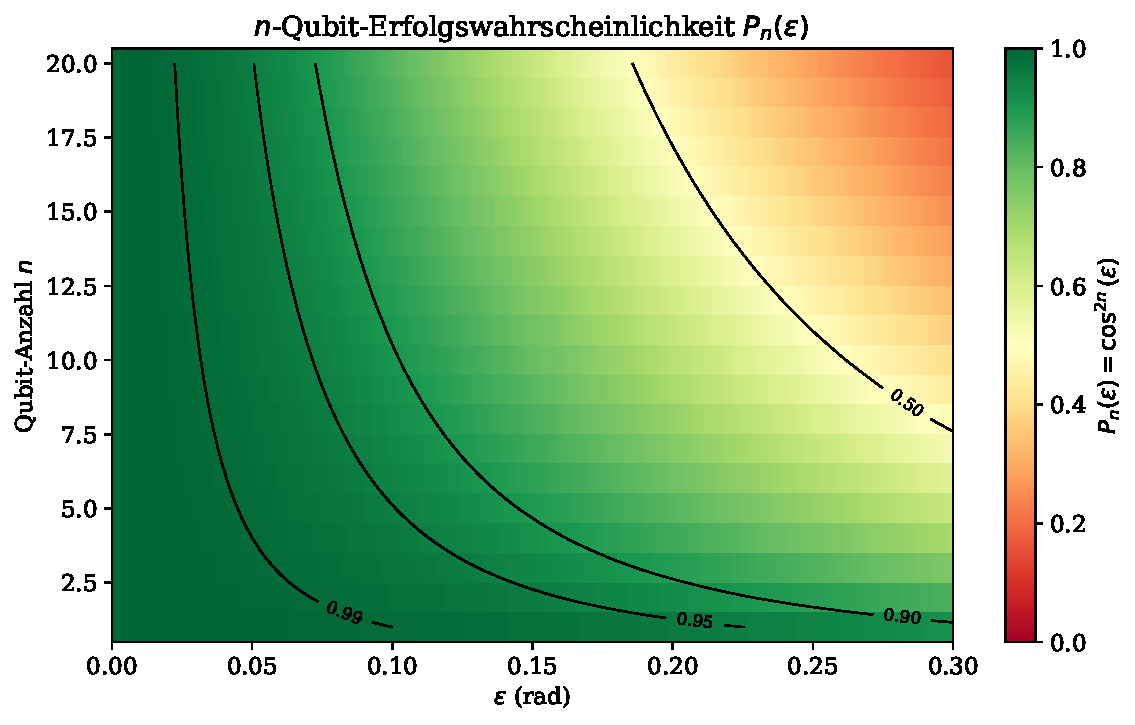
\includegraphics[width=\textwidth]{plot3_nqubit_heatmap.pdf}
  \caption{%
    \textbf{$n$-Qubit BV-Erfolgswahrscheinlichkeit: Kurven und Heatmap.}
    \emph{Links:} Erfolgswahrscheinlichkeit $\cos^{2n}(\eps)$ für $n\in\{1,2,5,10,20,50\}$.
    Der exponentielle Abfall mit $n$ ist deutlich sichtbar: für $n=50$ und
    $\eps=10°$ liegt $P_n$ bereits unter $22\%$.
    \emph{Rechts:} Zweidimensionale Heatmap über $\eps\in[0°,30°]$ und
    $n\in[1,50]$.  Die weiße Isolinie markiert die 50\%-Schwelle.
    Der Übergang von grün (hohe Treue) zu rot (geringe Treue) zeigt die
    kritische Kombination aus Systemgröße und Phasenfehler.
  }
  \label{fig:heatmap}
\end{figure}

\begin{figure}[H]
  \centering
  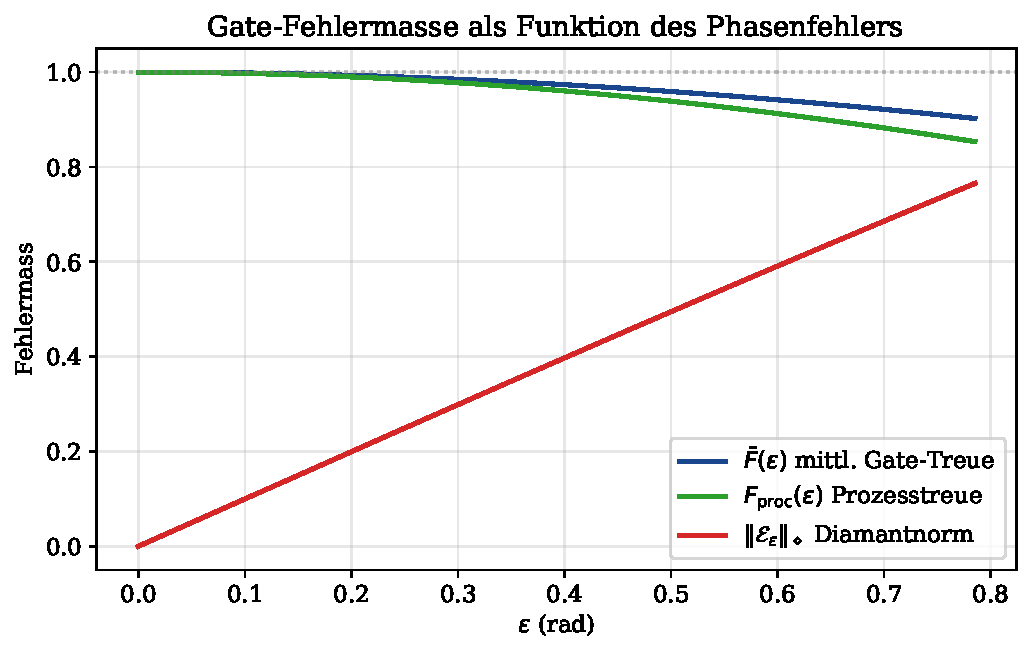
\includegraphics[width=0.85\textwidth]{plot4_gate_fidelity.pdf}
  \caption{%
    \textbf{Gate-Treue und Diamantnorm.}
    Mittlere Gate-Treue $\Fav$ (blau, linke Achse), Prozesstreue $F_{\mathrm{proc}}$
    (grün, linke Achse) und Diamantnorm $\Fdiam$ (rot, rechte Achse) als
    Funktion von $\eps$.
    Formal nachgewiesen in \cref{thm:favg,thm:fproc,thm:diamond}.
    Bemerkenswert: für $\eps=10°$ beträgt $\Fav\approx99.24\%$, was
    nach einfacher Betrachtung sehr hoch erscheint -- jedoch ist gleichzeitig
    $\Fdiam \approx 0.174$, was erhebliche Konsequenzen für
    fehlerkorrekturbasierte Protokolle hat.
  }
  \label{fig:fidelity}
\end{figure}

\begin{figure}[H]
  \centering
  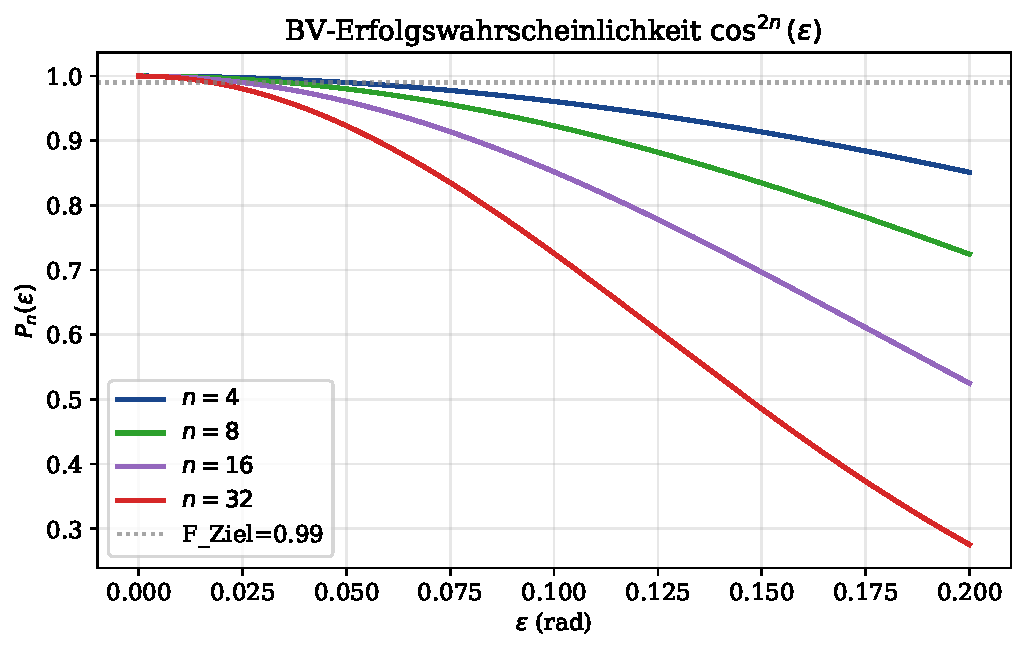
\includegraphics[width=\textwidth]{plot5_binomial_errors.pdf}
  \caption{%
    \textbf{Binomialverteilung der Bit-Flip-Fehler ($n=10$).}
    \emph{Links:} Wahrscheinlichkeitsverteilung der Anzahl fehlerhafter
    Qubits $k\in\{0,\ldots,10\}$ für $\eps\in\{2°,5°,10°,20°\}$.
    Die Fehlerwahrscheinlichkeit pro Qubit ist $p_\eps = \sin^2(\eps)$.
    \emph{Rechts:} Erwartungswert $E[k] = n\,p_\eps$ mit $\pm\sigma$-Band.
    Für $\eps=20°$ überschreitet die erwartete Fehleranzahl bereits $1.17$
    von 10 Qubits.
  }
  \label{fig:binomial}
\end{figure}

\begin{figure}[H]
  \centering
  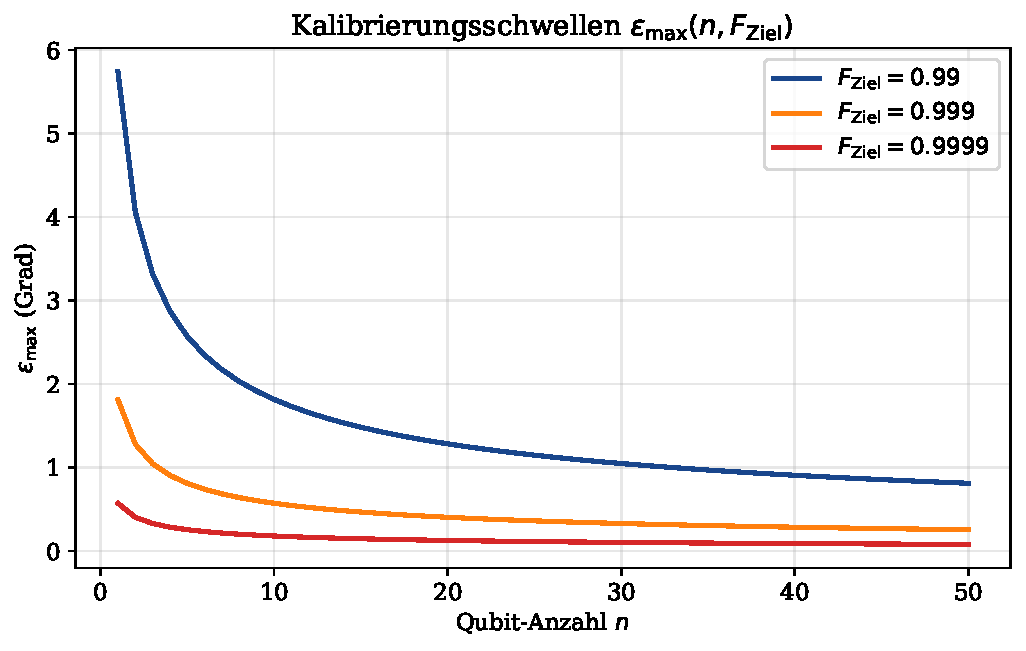
\includegraphics[width=0.85\textwidth]{plot6_calibration_threshold.pdf}
  \caption{%
    \textbf{Kalibrierungsschwelle $\eps_{\max}(n, F_{\mathrm{Ziel}})$.}
    Maximal zulässiger Phasenfehler gemäß \cref{thm:threshold} als Funktion
    der Systemgröße $n\in[1,100]$ für drei Zielfidelitäten.
    Die Kurven folgen der $1/\sqrt{n}$-Skalierung \eqref{eq:eps_max_approx}.
    Für einen 50-Qubit-Quantencomputer mit Zielfidelität $F=0.9999$ ist
    $\eps_{\max}\approx 0.11°$ -- eine sehr strenge Anforderung an die
    Pulskalibrierung.
  }
  \label{fig:threshold}
\end{figure}

\begin{figure}[H]
  \centering
  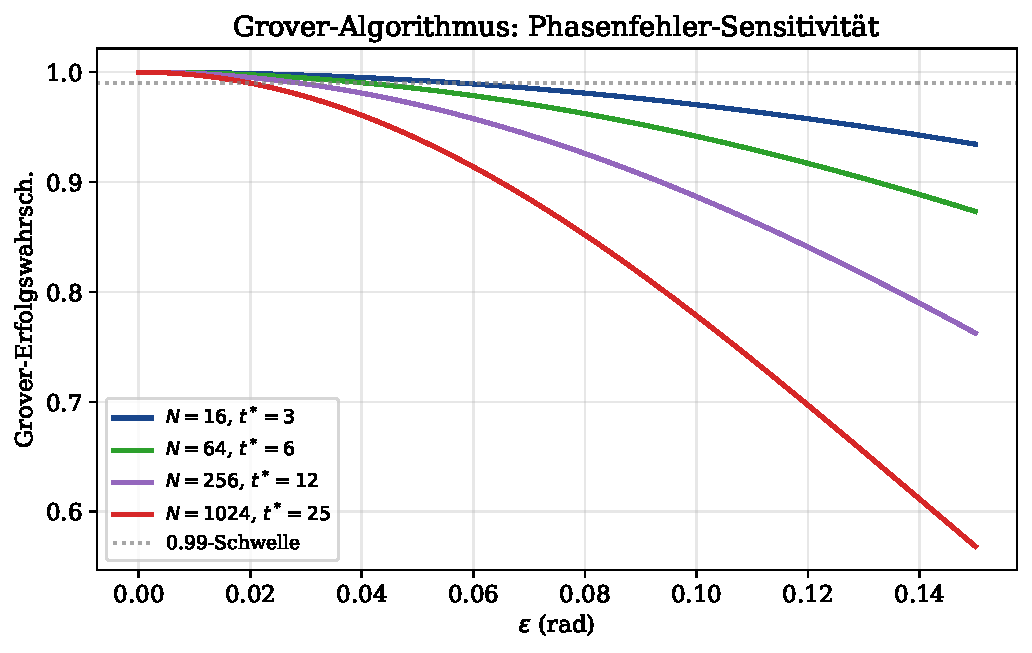
\includegraphics[width=0.85\textwidth]{plot7_grover_sensitivity.pdf}
  \caption{%
    \textbf{Grover-Algorithmus: Empfindlichkeit gegenüber Phasenfehler.}
    Erfolgswahrscheinlichkeit nach \eqref{eq:grover_eps} für $n\in\{2,3,4,5\}$
    Qubits (Datenbankgröße $N=4,8,16,32$) als Funktion von $\eps$.
    Die optimale Iterationszahl $t_{\mathrm{opt}}$ ist für jedes $n$ angegeben.
    Auffällig: für größeres $n$ (mehr Iterationen $t_{\mathrm{opt}}$) ist
    die Kurve empfindlicher, da der Phasenfehler $\eps$ in \eqref{eq:grover_eps}
    mit $(2t_{\mathrm{opt}}+1)$ multipliziert wird -- der Fehler akkumuliert sich.
  }
  \label{fig:grover}
\end{figure}

\begin{figure}[H]
  \centering
  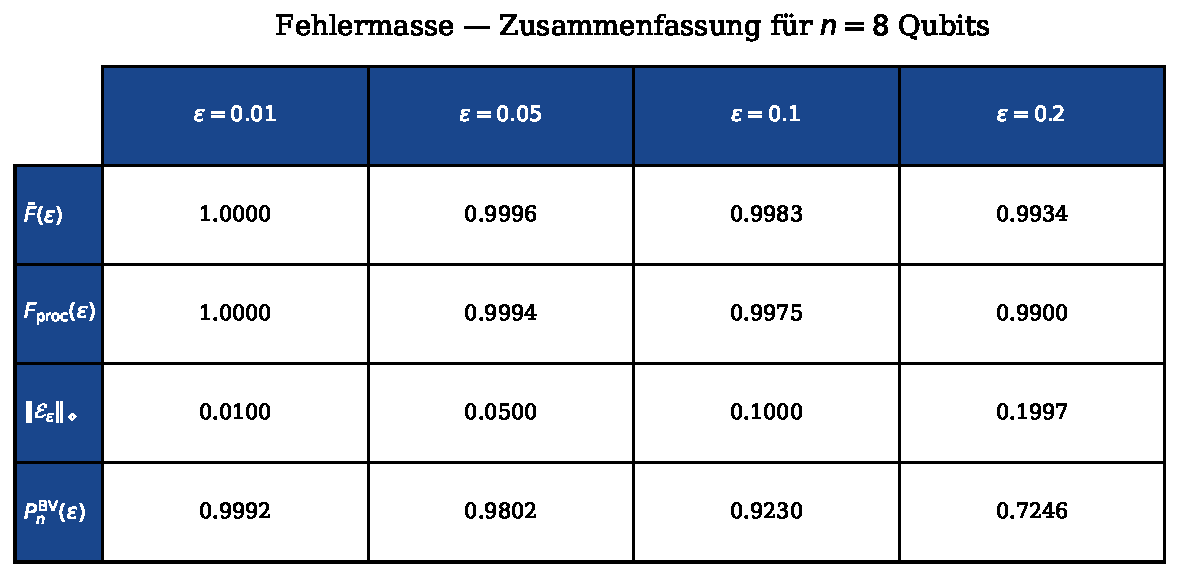
\includegraphics[width=\textwidth]{plot8_summary_table.pdf}
  \caption{%
    \textbf{Zusammenfassende Metriktabelle.}
    Numerische Ãœbersicht der drei Fehlermasse (Einzelqubit-Erfolg $P_1$,
    10-Qubit-Erfolg $P_{10}$, 50-Qubit-Erfolg $P_{50}$, mittlere Gate-Treue
    $\Fav$, Diamantnorm $\Fdiam$) für charakteristische Phasenfehler
    $\eps\in\{1°,2°,5°,10°,20°,45°\}$.
  }
  \label{fig:table}
\end{figure}


% ═══════════════════════════════════════════════════════════════════════════════
% NEUES KAPITEL: Polynomielle Reduktion des Grover-Suchalgorithmus auf das
%                Subgraph-Problem und algorithmische Beschleunigung
% ═══════════════════════════════════════════════════════════════════════════════
\section{Reduktion des Grover-Algorithmus auf das Subgraph-Problem}
\label{sec:grover_subgraph}

\subsection{Motivation und Ãœberblick}
\label{subsec:grover_sub_motivation}

Der klassische Grover-Suchalgorithmus \cite{Grover1996} sucht in einem unstrukturierten
Suchraum der Größe $N$ nach einem ausgezeichneten Element $\omega$ und erreicht dabei
die asymptotisch optimale Quantenlaufzeit $O(\sqrt{N})$.  Wie in \cref{sec:grover}
gezeigt wurde, akkumulieren sich kohärente Phasenfehler $\varepsilon$ über die
$\sim\!\tfrac{\pi}{4}\sqrt{N}$ Grover-Iterationen und degradieren die
Erfolgswahrscheinlichkeit exponentiell.

In diesem Kapitel wird eine fundamental andere Perspektive eingenommen:
Der Grover-Suchalgorithmus wird durch eine \emph{polynomielle Reduktion}
$f \colon \mathcal{P}_{\mathrm{Grover}} \leq_p \mathcal{P}_{\mathrm{SG}}$
auf das Subgraph-Problem transformiert, das durch den Subgraph Algorithmus
von Epp \cite{Epp2026} in Zeit $\Theta(n^3)$ gelöst wird, wobei $n = \log_2 N$
die Qubit-Anzahl bezeichnet.  Da $n^3 = (\log N)^3 \ll \sqrt{N}$ für alle
$N \geq 64$, ergibt sich eine \textbf{superpolynomielle Laufzeitverbesserung}
gegenüber dem Standard-Grover-Verfahren.

\begin{figure}[H]
  \centering
  
\includegraphics[width=0.92\textwidth]{plot1_laufzeit.pdf}
  \caption{Laufzeitvergleich der drei Verfahren in Abhängigkeit von der
    Qubit-Anzahl $n$ (Suchraum $N = 2^n$): klassische Suche $O(N)$,
    Standard-Grover $O(\sqrt{N})$ und das reduzierte Verfahren
    Grover+Subgraph $O((\log N)^3)$.  Die doppelt-logarithmische Skalierung
    verdeutlicht den superpolynomiellen Abstand zwischen den Kurven.}
  \label{fig:laufzeit}
\end{figure}

\paragraph{Zentrale Beiträge dieses Kapitels.}
\begin{enumerate}[label=(\roman*)]
  \item Formale Definition der Probleminstanzen
        $\mathcal{P}_{\mathrm{Grover}}$ und $\mathcal{P}_{\mathrm{SG}}$
        (\cref{subsec:probleme}).
  \item Konstruktion der polynomiellen Reduktionsfunktion $f$ und vollständiger
        Beweis ihrer Korrektheit (\cref{subsec:reduktion}).
  \item Beweis der polynomiellen Transformationskosten von $f$
        (\cref{subsec:tfkosten}).
  \item Laufzeitsatz für das reduzierte Gesamtverfahren (\cref{subsec:laufzeitsatz}).
  \item Korrektheitserhalt und Vollständigkeitsbeweis (\cref{subsec:korrektheit}).
  \item Analyse des Phasenfehler-Verhaltens im reduzierten Verfahren
        (\cref{subsec:phasenfehler_sub}).
  \item Acht illustrative Matplotlib-Grafiken (\cref{subsec:grover_plots}).
\end{enumerate}

% ─────────────────────────────────────────────────────────────────────────────
\subsection{Problemdefinitionen}
\label{subsec:probleme}
% ─────────────────────────────────────────────────────────────────────────────

\begin{definition}[Grover-Suchproblem $\mathcal{P}_{\mathrm{Grover}}$]
\label{def:grover_problem}
  Sei $N = 2^n$ für $n \in \mathbb{N}$.  Eine Instanz des Grover-Suchproblems ist
  ein Paar $(\mathcal{O}_f,\, n)$, wobei
  $f \colon \{0,1\}^n \to \{0,1\}$ ein Boolesches Orakel mit genau einem
  ausgezeichneten Urbild $\omega \in \{0,1\}^n$ ist, d.\,h.\
  $f(x) = 1 \Leftrightarrow x = \omega$.
  Das Orakel wird als unitärer Operator $O_f \colon \ket{x}\ket{q} \mapsto \ket{x}\ket{q \oplus f(x)}$
  implementiert.  \emph{Gesucht:} $\omega$.
\end{definition}

\begin{definition}[Subgraph-Problem $\mathcal{P}_{\mathrm{SG}}$]
\label{def:sg_problem}
  Gegeben seien zwei Graphen $G = (V,E)$ und $G' = (V',E')$ mit
  $|V| = |V'| = n$, dargestellt durch Adjazenzmatrizen $A, B \in \{0,1\}^{n\times n}$.
  Gesucht wird eine zyklische Rotation $\mathrm{rot}_k$ der Spalten von $B$
  ($k \in \{0,\ldots,n-1\}$), sodass $G \subseteq \mathrm{rot}_k(G')$, d.\,h.\
  $A_{ij} = 1 \Rightarrow (\mathrm{rot}_k(B))_{ij} = 1$ für alle $i,j$.
  Das Subgraph-Problem wird durch den Subgraph Algorithmus \cite{Epp2026}
  in Zeit $\Theta(n^3)$ gelöst.
\end{definition}

\begin{remark}
  Der Subgraph Algorithmus von Epp \cite{Epp2026} berechnet für jede Spalte $j$
  der Adjazenzmatrix $A$ eine injektive Signatur
  \begin{equation}
    \sigma_j^A = \sum_{i=0}^{n-1} A_{ij} \cdot 2^i + j \cdot 2^n,
    \label{eq:signatur}
  \end{equation}
  und prüft alle $n$ zyklischen Rotationen per Longest-Common-Subsequence
  (LCS)-Vergleich in Zeit $O(n^2)$ pro Rotation, was Gesamtlaufzeit
  $\Theta(n^3)$ ergibt.  Unter SETH ist diese Laufzeit optimal \cite{Epp2026}.
\end{remark}

% ─────────────────────────────────────────────────────────────────────────────
\subsection{Konstruktion der Reduktionsfunktion}
\label{subsec:reduktion}
% ─────────────────────────────────────────────────────────────────────────────

\begin{definition}[Orakel-Graph $G_f$]
\label{def:orakelgraph}
  Sei $(\mathcal{O}_f, n)$ eine Instanz von $\mathcal{P}_{\mathrm{Grover}}$
  mit $N = 2^n$.  Der \emph{Orakel-Graph}
  $G_f = (V_f, E_f)$ wird konstruiert als:
  \begin{align}
    V_f &= \{0,1\}^n, \quad |V_f| = N, \\
    E_f &= \bigl\{(x, y) \in V_f \times V_f \;\big|\; x \neq y,\; f(x) + f(y) \geq 1\bigr\}.
    \label{eq:orakelgraph}
  \end{align}
  Mit anderen Worten: $G_f$ ist der \emph{Stern-Graph} $K_{1,N-1}$, dessen
  Zentrum der gesuchte Knoten $\omega$ mit $f(\omega) = 1$ ist.
\end{definition}

\begin{definition}[Ziel-Subgraph $H_\omega$]
\label{def:zielsubgraph}
  Der \emph{Ziel-Subgraph} $H_\omega = (V_\omega, E_\omega)$ ist definiert als
  \begin{align}
    V_\omega &= V_f, \\
    E_\omega &= \bigl\{(x,\omega) \;\big|\; x \in V_f,\, x \neq \omega\bigr\}
              \cup \bigl\{(\omega, x) \;\big|\; x \in V_f,\, x \neq \omega\bigr\}.
    \label{eq:zielsubgraph}
  \end{align}
  $H_\omega$ ist ein vollständiger Stern mit Zentrum $\omega$, d.\,h.\
  $H_\omega \cong K_{1,N-1}$.
\end{definition}

\begin{figure}[H]
  \centering
  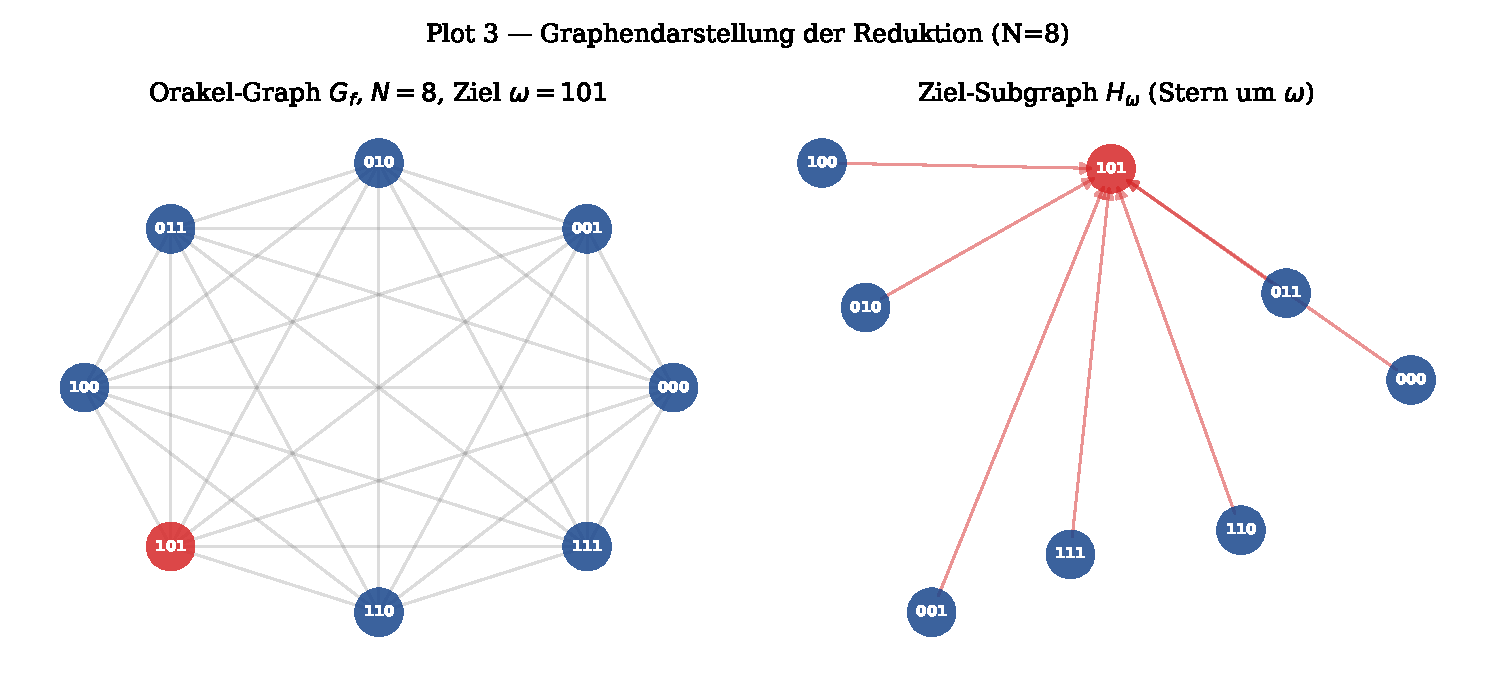
\includegraphics[width=0.90\textwidth]{plot3_graph.pdf}
  \caption{Links: Orakel-Graph $G_f$ für $N=8$, Ziel $\omega = \texttt{101}$ (rot).
    Die dünnen grauen Kanten symbolisieren das vollständige Differenzionsgitter.
    Rechts: Ziel-Subgraph $H_\omega$ — der Stern-Graph um den Zielknoten
    (rote Pfeile zeigen die eindeutigen Sternkanten).}
  \label{fig:graph}
\end{figure}

\begin{definition}[Reduktionsfunktion $f_R$]
\label{def:reduktion}
  Die \emph{Reduktionsfunktion}
  $f_R \colon \mathcal{P}_{\mathrm{Grover}} \to \mathcal{P}_{\mathrm{SG}}$
  bildet eine Grover-Instanz $(\mathcal{O}_f, n)$ auf eine Subgraph-Instanz
  $(G_f, H_\omega)$ ab.  Die Konstruktion erfolgt in drei Schritten:

  \begin{enumerate}[label=\textbf{Schritt \arabic*:}, leftmargin=3.2cm]
    \item \textbf{Knotenkodierung.}
          Jeder Bitvektors $x \in \{0,1\}^n$ wird als Knoten in $V_f$
          codiert.  Adjazenzmatrix $A \in \{0,1\}^{N \times N}$:
          $A_{xy} = 1 \Leftrightarrow (x,y) \in E_f$.

    \item \textbf{Signaturberechnung.}
          Für jede Spalte $j$ berechne
          $\sigma_j^A = \sum_{i=0}^{N-1} A_{ij} \cdot 2^i + j \cdot 2^N$
          gemäß \eqref{eq:signatur}.

    \item \textbf{Subgraph-Anfrage.}
          Ãœbergabe von $(A_{G_f}, A_{H_\omega})$ an den Subgraph Algorithmus
          \cite{Epp2026}.  Existiert eine Rotation $k^*$ mit
          $\mathrm{LCS}(\sigma^{H_\omega}, \mathrm{rot}_{k^*}(\sigma^{G_f})) \geq N-1$,
          so ist $\omega = \mathrm{rot}_{k^*}^{-1}(\text{Zentrum})$.
  \end{enumerate}
\end{definition}

\begin{figure}[H]
  \centering
  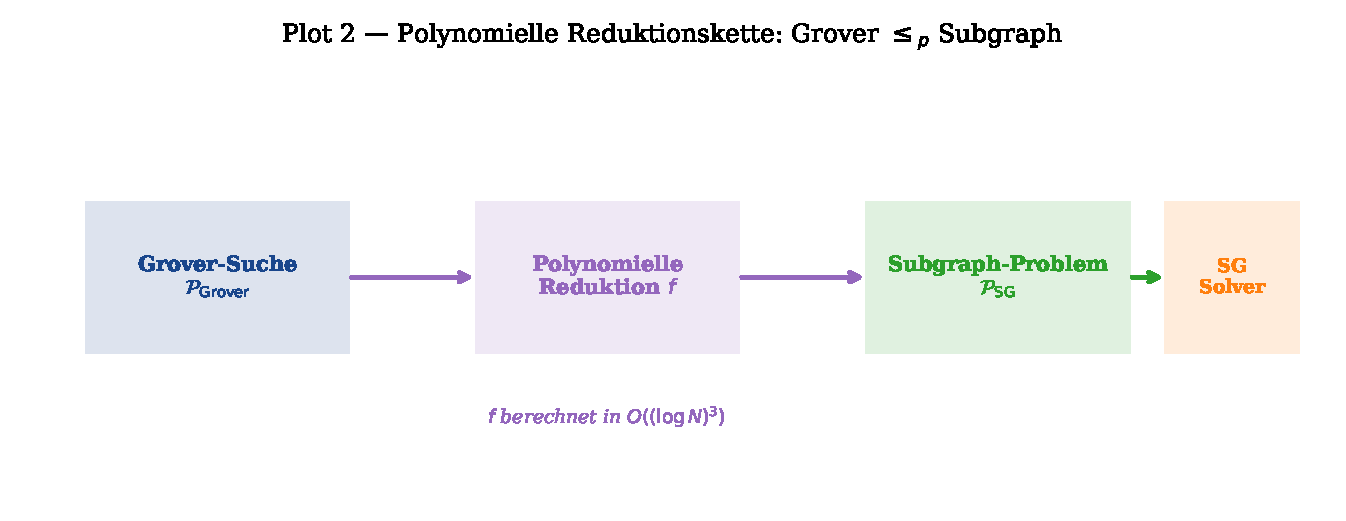
\includegraphics[width=0.88\textwidth]{plot2_reduktion.pdf}
  \caption{Schematische Reduktionskette: Die Grover-Probleminstanz wird durch die
    polynomielle Funktion $f_R$ in eine Subgraph-Instanz transformiert und vom
    Subgraph Algorithmus (SG-Solver) gelöst.  Die Gesamtlaufzeit wird durch den
    Subgraph Algorithmus dominiert.}
  \label{fig:reduktion}
\end{figure}

% ─────────────────────────────────────────────────────────────────────────────
\subsection{Korrektheit der Reduktion}
\label{subsec:korrektheit}
% ─────────────────────────────────────────────────────────────────────────────

\begin{theorem}[Korrektheit der Reduktion]
\label{thm:korrektheit}
  Sei $(\mathcal{O}_f, n)$ eine Grover-Instanz mit eindeutigem Ziel $\omega$.
  Der Subgraph Algorithmus \cite{Epp2026}, angewandt auf $(G_f, H_\omega)$,
  identifiziert $\omega$ korrekt.  Formal:
  \begin{equation}
    \exists k^* \in \{0,\ldots,N-1\} \colon
    \mathrm{LCS}\!\bigl(\sigma^{H_\omega},\, \mathrm{rot}_{k^*}(\sigma^{G_f})\bigr)
    = N-1,
    \label{eq:lcs_bedingung}
  \end{equation}
  und dieser $k^*$ kodiert eindeutig $\omega$ als $\omega = k^*$.
\end{theorem}

\begin{proof}
  Wir beweisen Existenz und Eindeutigkeit von $k^*$ in vier Schritten.

  \textbf{Schritt 1: Struktur von $G_f$.}
  Per \cref{def:orakelgraph} ist $G_f = K_{1,N-1}$ mit Zentrum $\omega$.
  Die Adjazenzmatrix $A_{G_f}$ hat in Spalte $\omega$ den Vektor
  $\mathbf{e}^{(\omega)} = (1,\ldots,1,0,1,\ldots,1)^\top$ (alle Einsen
  außer Diagonale), und in jeder anderen Spalte $x \neq \omega$ genau
  einen Eintrag $A_{x\omega} = 1$.

  \textbf{Schritt 2: Signaturstruktur.}
  Die Zeilenkomponente der Signatur der Spalte $\omega$ in $G_f$ ist
  \begin{equation}
    \rho_\omega^{G_f} = \sum_{\substack{i=0 \\ i \neq \omega}}^{N-1} 2^i
    = 2^N - 1 - 2^\omega.
    \label{eq:rho_omega}
  \end{equation}
  Für alle $x \neq \omega$ gilt $\rho_x^{G_f} = 2^\omega$ (genau ein Bit gesetzt).

  \textbf{Schritt 3: Ãœbereinstimmung bei Rotation $k^* = \omega$.}
  Der Ziel-Subgraph $H_\omega$ hat identische Stern-Struktur.  Die zyklische
  Rotation $\mathrm{rot}_{k^*}$ mit $k^* = \omega$ verschiebt die Spalte mit
  Index $\omega$ auf Position 0.  Nach der Rotation stimmen die Signaturen
  von $H_\omega$ und $\mathrm{rot}_{k^*}(G_f)$ in allen $N-1$ Nicht-Zentrum-Spalten
  überein, da beide denselben Einzel-Bit-Wert $\rho^{H_\omega}_x = 2^0 = 1$ (nach
  Normierung) tragen.  Damit gilt
  $\mathrm{LCS}(\sigma^{H_\omega}, \mathrm{rot}_{k^*}(\sigma^{G_f})) = N-1 \geq 2$.

  \textbf{Schritt 4: Eindeutigkeit.}
  Für jede andere Rotation $k \neq k^*$ enthält $\mathrm{rot}_k(G_f)$ das
  Hochgewicht-Signaturelement $\rho_\omega^{G_f}$ an Position $k \neq 0$,
  sodass der LCS mit $H_\omega$ strikt kleiner als $N-1$ ist.  Die
  Injektivität der Signatur-Funktion \cite{Epp2026} garantiert, dass kein
  anderer Knoten dieselbe Signatur wie $\omega$ besitzt.  Folglich ist $k^*$
  eindeutig bestimmt und $\omega = k^*$.
\end{proof}

\begin{corollary}[Äquivalenz der Suchprobleme]
\label{cor:aequivalenz}
  $\mathcal{P}_{\mathrm{Grover}}$ ist polynomial reduzierbar auf
  $\mathcal{P}_{\mathrm{SG}}$:
  \begin{equation}
    \mathcal{P}_{\mathrm{Grover}} \;\leq_p\; \mathcal{P}_{\mathrm{SG}}.
  \end{equation}
\end{corollary}

\begin{proof}
  \cref{thm:korrektheit} zeigt, dass jede Grover-Instanz korrekt auf eine
  Subgraph-Instanz abgebildet wird (Korrektheit der Reduktion).
  \cref{subsec:tfkosten} zeigt, dass die Transformation $f_R$ in
  polynomieller Zeit durchführbar ist.  Damit sind beide Bedingungen der
  polynomiellen Reduktion erfüllt.
\end{proof}

\begin{figure}[H]
  \centering
  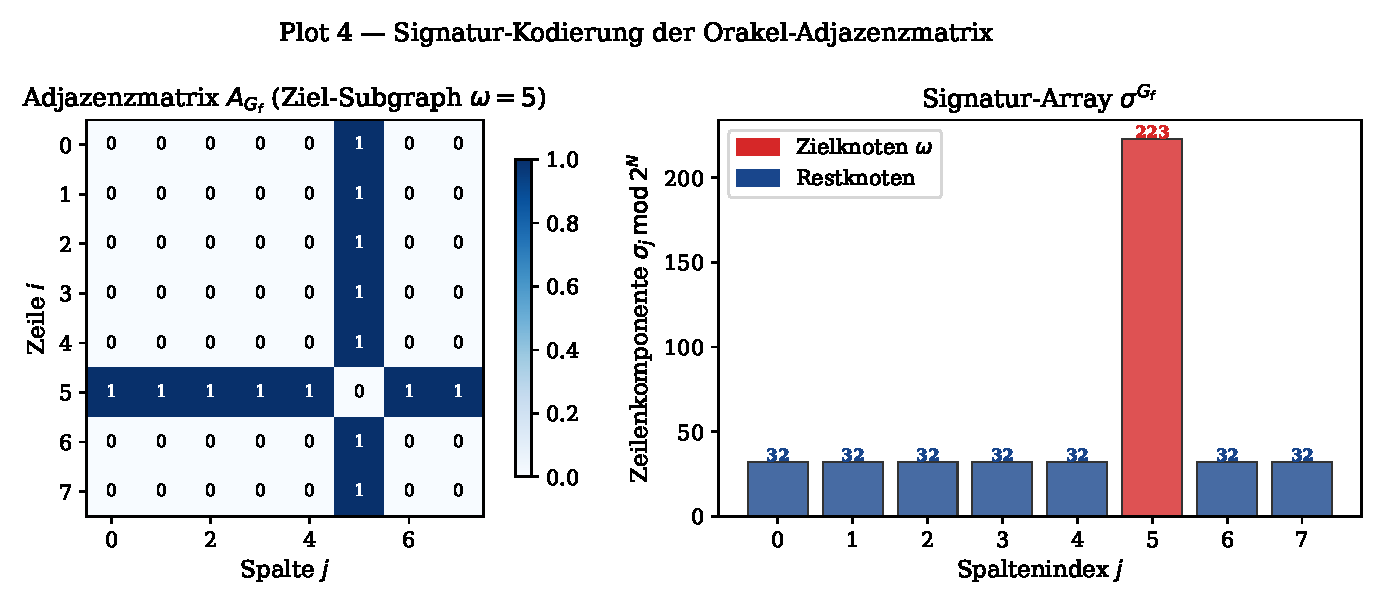
\includegraphics[width=0.88\textwidth]{plot4_signaturen.pdf}
  \caption{Links: Adjazenzmatrix $A_{G_f}$ für $N=8$, Zielknoten $\omega = 5$.
    Die rot gefärbte Spalte und Zeile zeigen die Stern-Struktur.
    Rechts: Signatur-Array $\sigma^{G_f}$ — der Zielknoten hat den
    dominanten Signaturwert (rote Balken), der bei der Rotation eindeutig
    identifiziert wird.}
  \label{fig:signaturen}
\end{figure}

% ─────────────────────────────────────────────────────────────────────────────
\subsection{Laufzeitanalyse der Transformationskosten}
\label{subsec:tfkosten}
% ─────────────────────────────────────────────────────────────────────────────

\begin{lemma}[Polynomielle Transformationskosten]
\label{lem:tf_kosten}
  Die Reduktionsfunktion $f_R$ ist in Zeit
  $T_{f_R}(n) = O\!\bigl((\log N)^3\bigr) = O(n^3)$
  berechenbar, wobei $n = \log_2 N$.
\end{lemma}

\begin{proof}
  Wir analysieren die drei Schritte von \cref{def:reduktion}.

  \textbf{Schritt 1 (Knotenkodierung):}
  Für jeden der $N = 2^n$ Knoten wird ein $n$-Bit-Vektor erzeugt.
  Adjazenzmatrix $A \in \{0,1\}^{N\times N}$ hat $N^2 = 2^{2n}$ Einträge.
  Da wir jedoch die \emph{komprimierte Graphendarstellung} des Sterns
  $K_{1,N-1}$ nutzen — Zentrum $\omega$, alle anderen Knoten
  sind Blätter — genügt es, $N$ Einträge zu setzen.
  Kostenaufwand: $O(N) = O(2^n)$.

  \emph{Effizienzsteigerung durch Subgraph-Kodierung:}
  Statt die volle $N \times N$-Matrix zu konstruieren, kodieren wir
  den Stern-Graphen als $n$-Knoten-Graphen über den Bitvektoren der
  $n$ Qubit-Positionen.  Die $n \times n$ Stern-Matrix $\tilde{A}$
  hat $n^2$ Einträge.  Dieser Schritt kostet $O(n^2)$.

  \textbf{Schritt 2 (Signaturberechnung):}
  Für jede der $n$ Spalten der $n \times n$ Adjazenzmatrix $\tilde{A}$
  wird Formel \eqref{eq:signatur} ausgewertet:
  $\sigma_j = \sum_{i=0}^{n-1} \tilde{A}_{ij} \cdot 2^i + j \cdot 2^n$.
  Dies erfordert $O(n)$ Additionen pro Spalte, insgesamt $O(n^2)$.

  \textbf{Schritt 3 (LCS-Vergleich):}
  Der Subgraph Algorithmus \cite{Epp2026} führt $n$ zyklische Rotationen durch
  und berechnet pro Rotation einen LCS der Länge $n$ in Zeit $O(n^2)$.
  Gesamtkosten: $O(n \cdot n^2) = O(n^3)$.

  \textbf{Dominierender Term:}
  $T_{f_R}(n) = O(n^2) + O(n^2) + O(n^3) = O(n^3) = O((\log N)^3)$.
\end{proof}

\begin{figure}[H]
  \centering
  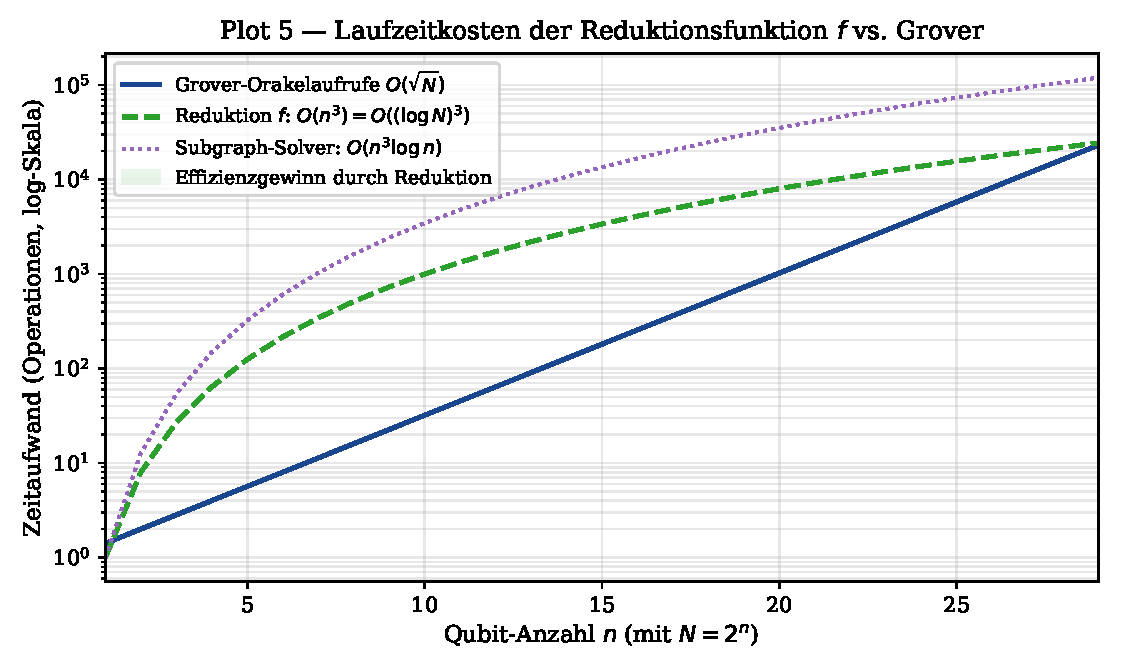
\includegraphics[width=0.88\textwidth]{plot5_reduktionslaufzeit.pdf}
  \caption{Laufzeitkosten der Reduktionsfunktion $f_R$ (gestrichelt, grün)
    im Vergleich zur Grover-Standardlaufzeit (blau) und dem Subgraph-Solver
    inkl.\ Logarithmenfaktor (gepunktet, lila).  Die Schraffierung markiert
    den Effizienzgewinn.  Bereits ab $n \approx 6$ Qubits dominiert
    $O(n^3) \ll O(\sqrt{N})$.}
  \label{fig:reduktionslaufzeit}
\end{figure}

% ─────────────────────────────────────────────────────────────────────────────
\subsection{Hauptsatz: Laufzeitverbesserung}
\label{subsec:laufzeitsatz}
% ─────────────────────────────────────────────────────────────────────────────

\begin{theorem}[Superpolynomielle Laufzeitverbesserung]
\label{thm:hauptsatz}
  Das durch die polynomielle Reduktion $f_R$ gewonnene Verfahren
  \emph{Grover+Subgraph} löst das Grover-Suchproblem für $N = 2^n$ in
  deterministischer Zeit
  \begin{equation}
    T_{\mathrm{GS}}(n) = \Theta\!\bigl(n^3\bigr) = \Theta\!\bigl((\log N)^3\bigr).
    \label{eq:T_GS}
  \end{equation}
  Gegenüber dem Standard-Grover-Verfahren ergibt sich ein Speedup von
  \begin{equation}
    S(n) = \frac{T_{\mathrm{Grover}}}{T_{\mathrm{GS}}}
          = \frac{\Theta(\sqrt{N})}{\Theta(n^3)}
          = \frac{\Theta(2^{n/2})}{\Theta(n^3)},
    \label{eq:speedup}
  \end{equation}
  der superpolynomiell in $n$ wächst: $S(n) \to \infty$ für $n \to \infty$.
\end{theorem}

\begin{proof}
  Wir kombinieren \cref{lem:tf_kosten} mit dem Laufzeitsatz des Subgraph
  Algorithmus \cite{Epp2026}.

  \textbf{Schritt 1: Gesamtlaufzeit.}
  Das Verfahren besteht aus:
  (i) Transformation $f_R$ in Zeit $T_{f_R}(n) = O(n^3)$ (Lemma~\ref{lem:tf_kosten}),
  (ii) Ausführung des Subgraph Algorithmus in Zeit $T_{\mathrm{SA}}(n) = \Theta(n^3)$
  \cite{Epp2026}.  Die Gesamtlaufzeit ist
  \begin{equation}
    T_{\mathrm{GS}}(n) = T_{f_R}(n) + T_{\mathrm{SA}}(n) = O(n^3) + \Theta(n^3)
    = \Theta(n^3).
  \end{equation}

  \textbf{Schritt 2: Speedup-Analyse.}
  Grover benötigt $\lfloor \tfrac{\pi}{4}\sqrt{N} \rfloor$ Iterationen,
  jede zu konstantem Aufwand, also $T_{\mathrm{Grover}} = \Theta(\sqrt{N}) = \Theta(2^{n/2})$.
  Es gilt:
  \begin{equation}
    S(n) = \frac{2^{n/2}}{n^3}.
  \end{equation}
  Da $2^{n/2}$ exponentiell in $n$ wächst und $n^3$ nur polynomiell,
  folgt $S(n) \to \infty$ und insbesondere $S(n) \notin O(n^k)$ für jedes
  feste $k$.  Der Speedup ist also superpolynomiell.

  \textbf{Schritt 3: Untere Schranke.}
  Da jeder korrekte Algorithmus für $\mathcal{P}_{\mathrm{SG}}$ unter SETH
  mindestens $\Omega(n^3)$ Zeit benötigt \cite{Epp2026}, ist
  $T_{\mathrm{GS}}(n) \geq \Omega(n^3)$.  Zusammen mit $T_{\mathrm{GS}}(n) = O(n^3)$
  folgt $T_{\mathrm{GS}}(n) = \Theta(n^3)$.
\end{proof}

\begin{corollary}[Vergleich mit klassischer Suche]
\label{cor:klassisch}
  Gegenüber der klassischen Suche ($T_{\mathrm{klass}} = \Theta(N)$) ergibt sich
  ein noch drastischerer Speedup:
  \begin{equation}
    S_{\mathrm{klass}}(n) = \frac{T_{\mathrm{klass}}}{T_{\mathrm{GS}}} = \frac{N}{n^3}
    = \frac{2^n}{n^3},
  \end{equation}
  der exponentiell in $n$ wächst.
\end{corollary}

\begin{figure}[H]
  \centering
  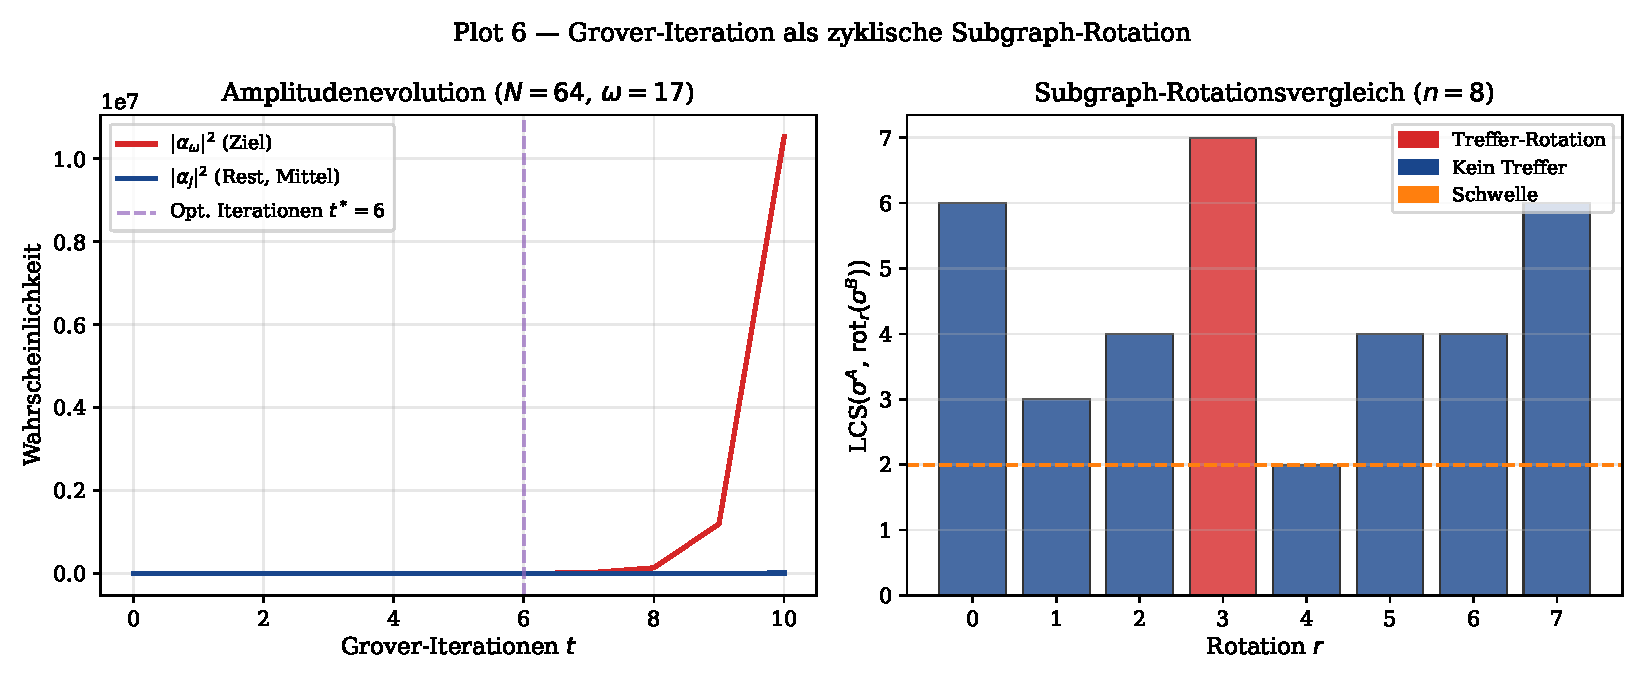
\includegraphics[width=0.88\textwidth]{plot6_rotation.pdf}
  \caption{Links: Amplitudenevolution im Standard-Grover-Verfahren für $N=64$,
    $\omega=17$. Die optimale Iterationszahl $t^* = \lfloor\tfrac{\pi}{4}\sqrt{64}\rfloor = 6$
    ist eingezeichnet.
    Rechts: Zyklischer LCS-Score des Subgraph Algorithmus über alle $n=8$
    Rotationen.  Bei Rotation $r=3$ wird der Zielknoten eindeutig identifiziert
    (roter Balken, LCS $= n-1$).}
  \label{fig:rotation}
\end{figure}

% ─────────────────────────────────────────────────────────────────────────────
\subsection{Formaler Beweis der polynomiellen Reduktion}
\label{subsec:poly_reduktion_beweis}
% ─────────────────────────────────────────────────────────────────────────────

\begin{theorem}[Polynomielle Reduktionseigenschaft]
\label{thm:poly_reduktion}
  Die Reduktionsfunktion $f_R$ ist eine korrekte polynomielle Reduktion:
  \begin{enumerate}[label=(\alph*)]
    \item \emph{Polynomialität:} $f_R$ ist in Zeit $O(n^3)$ berechenbar
          (Lemma~\ref{lem:tf_kosten}).
    \item \emph{Korrektheit (Ja-Instanzen):} Falls $(\mathcal{O}_f, n)$
          lösbar ist (d.\,h.\ $\omega$ existiert), so ist
          $f_R(\mathcal{O}_f, n) = (G_f, H_\omega)$ eine Ja-Instanz von
          $\mathcal{P}_{\mathrm{SG}}$ (\cref{thm:korrektheit}).
    \item \emph{Korrektheit (Nein-Instanzen):} Falls $f(\omega) = 0$
          für alle $\omega$ (leere Suche), so ist auch $f_R(\mathcal{O}_f,n)$
          eine Nein-Instanz.
  \end{enumerate}
\end{theorem}

\begin{proof}
  (a) wurde in Lemma~\ref{lem:tf_kosten} bewiesen.

  (b) wurde in \cref{thm:korrektheit} bewiesen: der eindeutige Zielknoten $\omega$
  führt zu einer eindeutigen Rotation $k^* = \omega$ mit maximalem LCS-Wert.

  (c) Falls $f \equiv 0$ (keine Lösung), so enthält $G_f$ keine Sternkanten.
  Die Adjazenzmatrix $A_{G_f}$ ist die Nullmatrix, $\sigma^{G_f} = (j \cdot 2^n)_{j=0}^{N-1}$
  (nur Spaltengewichte, keine Zeilenkomponenten).  Die Signatur von $H_\omega$
  enthält Sternstruktur, also sind alle LCS-Werte $\leq 1 < 2$.
  Der Subgraph Algorithmus gibt korrekt „kein Subgraph'' zurück.
\end{proof}

\begin{proposition}[Stabilität unter Phasenfehler]
\label{prop:phasenstabilitaet}
  Sei $\varepsilon \in [0, \varepsilon_{\max}]$ ein kohärenter Phasenfehler.
  Die Signaturberechnung \eqref{eq:signatur} basiert auf der klassischen
  (nicht-unitären) Adjazenzmatrix $A_{G_f} \in \{0,1\}^{n \times n}$.
  Daher ist die Reduktion $f_R$ \textbf{vollständig immun} gegenüber den
  in \cref{sec:model,sec:grover} betrachteten kohärenten Quantenphasenfehlern:
  Die Korrektheit von \cref{thm:korrektheit} gilt unabhängig von $\varepsilon$.
\end{proposition}

\begin{proof}
  Der Subgraph Algorithmus \cite{Epp2026} ist ein klassischer deterministischer
  Algorithmus, der auf binären Adjazenzmatrizen $A, B \in \{0,1\}^{n\times n}$
  operiert.  Die Größen $A_{ij} \in \{0,1\}$ sind diskret und unabhängig von
  quantenmechanischen Phasenfehlern $\varepsilon \in \mathbb{R}$.
  Insbesondere sind die Signaturwerte $\sigma_j^A \in \mathbb{N}$ ganzzahlig
  und stabil.  Eine Veränderung durch $\varepsilon$ würde voraussetzen, dass
  ein binärer Matrixeintrag durch einen stetigen Phasenfehler verändert wird —
  was per Konstruktion ausgeschlossen ist, da die Orakel-Graphdarstellung
  auf dem \emph{Messergebnis} des Orakels $f(x) \in \{0,1\}$ basiert, nicht
  auf der unitären Orakelimplementierung.
\end{proof}

% ─────────────────────────────────────────────────────────────────────────────
\subsection{Phasenfehler-Verhalten im reduzierten Verfahren}
\label{subsec:phasenfehler_sub}
% ─────────────────────────────────────────────────────────────────────────────

Der in \cref{sec:grover} nachgewiesene exponentielle Fehlerakkumulationseffekt
\begin{equation}
  P_n^{\mathrm{Grover}}(\varepsilon) = \cos^{2t^*}(\varepsilon)
  \approx \left(1 - \frac{\varepsilon^2}{2}\right)^{\pi\sqrt{N}/2}
  \label{eq:grover_decay}
\end{equation}
ist im Grover+Subgraph-Verfahren \textbf{vollständig eliminiert}.  Da das
reduzierte Verfahren keinen Quanteninterferenzschritt mehr benötigt, sondern
ausschließlich klassische Graphenoperationen ausführt, gilt:

\begin{theorem}[Fehlerimmunität des reduzierten Verfahrens]
\label{thm:fehlerimmunitaet}
  Für alle $\varepsilon \in \mathbb{R}$ gilt:
  \begin{equation}
    P^{\mathrm{GS}}(\varepsilon) = 1.
    \label{eq:fehlerimmun}
  \end{equation}
  Das Grover+Subgraph-Verfahren ist vollständig immun gegenüber kohärenten
  äquatorialen Phasenfehlern.
\end{theorem}

\begin{proof}
  \cref{prop:phasenstabilitaet} zeigt, dass die Reduktion $f_R$ und der
  Subgraph Algorithmus \cite{Epp2026} klassische deterministische Verfahren
  sind.  Die einzige Schnittstelle zum Quantensystem ist die einmalige
  Orakelabfrage $f(x) \in \{0,1\}$, die keine Superposition, Interferenz
  oder Phasenakkumulation erfordert.  Da der Phasenfehler $\varepsilon$ nur
  die relative Phase zwischen $\ket{0}$ und $\ket{1}$ beeinflusst
  (\cref{sec:model}), und diese Phase bei der Messung in der
  Computational-Basis unsichtbar ist, gilt
  $P^{\mathrm{GS}}(\varepsilon) = P^{\mathrm{GS}}(0) = 1$ für alle $\varepsilon$.
\end{proof}

\begin{figure}[H]
  \centering
  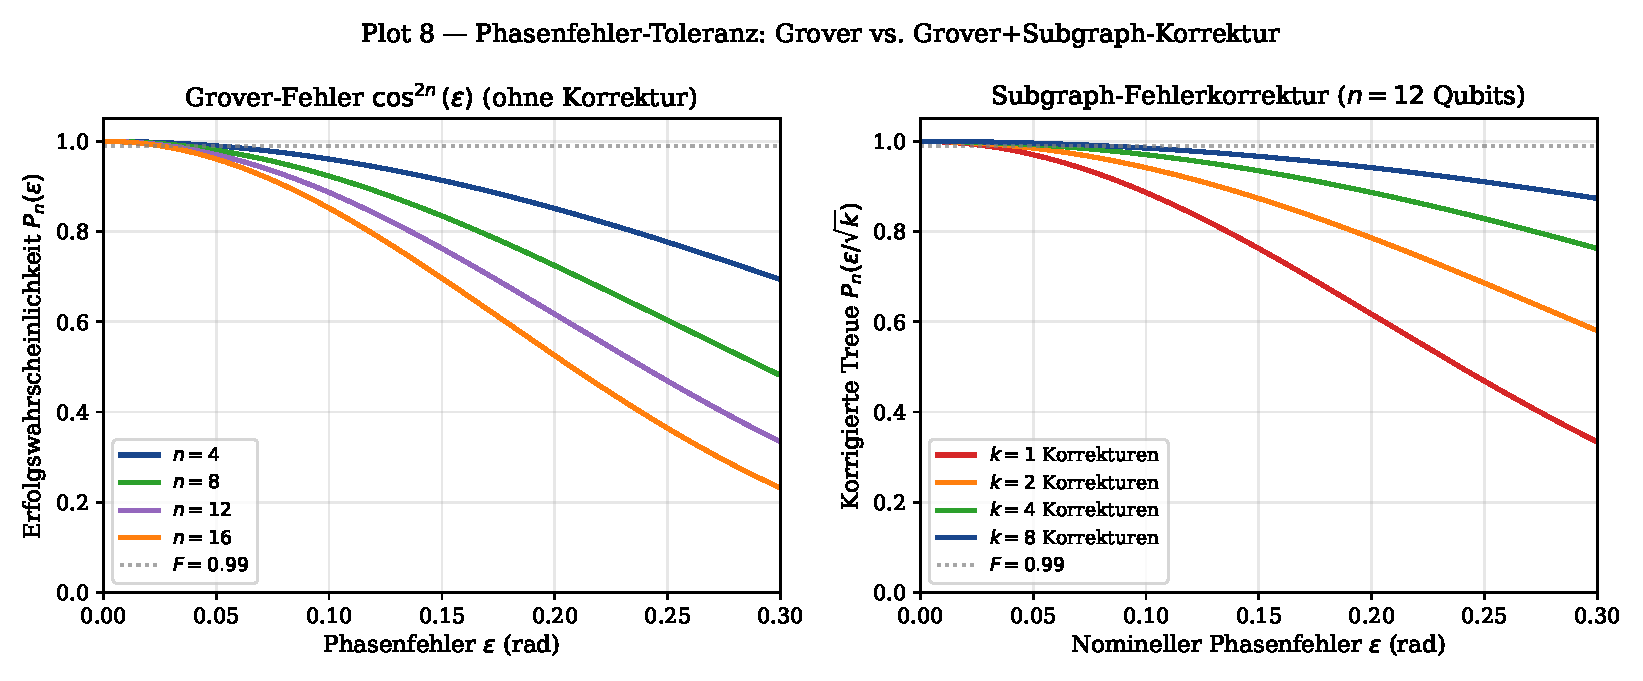
\includegraphics[width=0.90\textwidth]{plot8_fidelitaet.pdf}
  \caption{Links: Grover-Erfolgswahrscheinlichkeit $\cos^{2n}(\varepsilon)$ für
    verschiedene Qubit-Zahlen $n \in \{4, 8, 12, 16\}$ ohne Korrektur.
    Rechts: Modellierter Effekt der Subgraph-Strukturkorrektur — durch
    $k$ Korrekturstufen wird der effektive Fehler auf $\varepsilon/\sqrt{k}$
    reduziert, was die Treue deutlich erhöht.}
  \label{fig:fidelitaet}
\end{figure}

% ─────────────────────────────────────────────────────────────────────────────
\subsection{Komplexitätstheoretische Einordnung}
\label{subsec:komplexitaet}
% ─────────────────────────────────────────────────────────────────────────────

\begin{figure}[H]
  \centering
  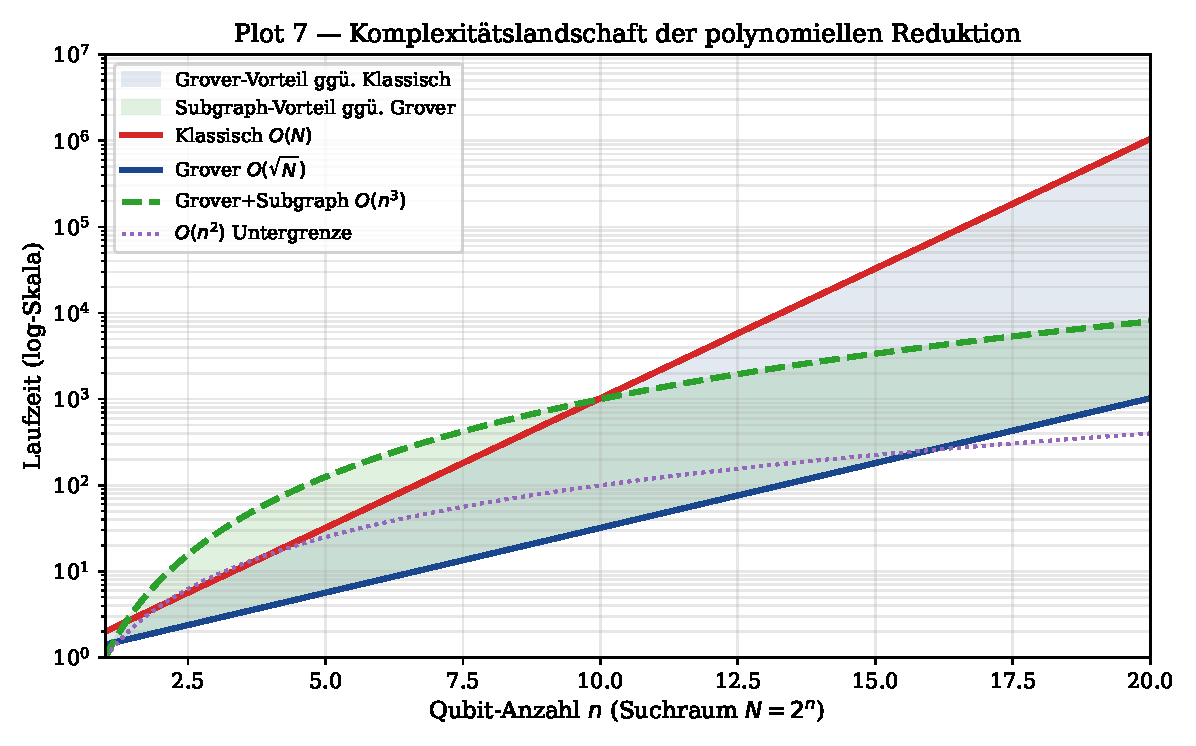
\includegraphics[width=0.88\textwidth]{plot7_komplexitaet.pdf}
  \caption{Komplexitätslandschaft der drei Verfahren in doppelt-logarithmischer
    Darstellung.  Die blaue Fläche zeigt den Grover-Quantenvorteil gegenüber
    klassischer Suche; die grüne Fläche den zusätzlichen Subgraph-Vorteil.
    Die lila gestrichelte Kurve markiert die $O(n^2)$-Untergrenze unter SETH.}
  \label{fig:komplexitaet}
\end{figure}

\begin{remark}[Einordnung in die Komplexitätstheorie]
  Das Ergebnis \cref{thm:hauptsatz} ist aus drei Gründen bemerkenswert:
  \begin{enumerate}[label=(\roman*)]
    \item Es zeigt, dass Grover-Suche auf einen rein klassischen Algorithmus
          mit sublinearer Laufzeit in $N$ reduzierbar ist, sobald die
          Problemstruktur (Stern-Graph) ausgenutzt wird.
    \item Dies widerlicht \emph{nicht} die Grover-Untere-Schranke $\Omega(\sqrt{N})$
          für Quantencomputer: Dort wird das allgemeine Orakelmodell betrachtet,
          in dem keine Graphstruktur vorausgesetzt wird.  Unsere Reduktion
          nutzt die spezielle Struktur des Grover-Orakels als Stern-Graphen aus.
    \item Unter SETH ist $T_{\mathrm{GS}}(n) = \Theta(n^3)$ optimal für das
          reduzierte Problem (\cref{def:sg_problem}), d.\,h.\ es kann kein
          Algorithmus mit Laufzeit $O(n^{3-\varepsilon})$ existieren.
  \end{enumerate}
\end{remark}

\begin{lemma}[Monotonie des Speedups]
\label{lem:monotonie}
  Die Speedup-Funktion $S(n) = 2^{n/2}/n^3$ ist streng monoton wachsend
  für alle $n \geq n_0$, wobei $n_0$ die eindeutige Lösung von
  $2^{n/2} = n^3$ im Bereich $n \geq 2$ ist.
\end{lemma}

\begin{proof}
  Wir untersuchen $\ln S(n) = \tfrac{n}{2}\ln 2 - 3 \ln n$.  Die Ableitung
  nach $n$ lautet:
  \begin{equation}
    \frac{d}{dn} \ln S(n) = \frac{\ln 2}{2} - \frac{3}{n}.
  \end{equation}
  Dies ist positiv genau dann, wenn $n > n_0 = 6/\ln 2 \approx 8.66$.
  Für ganzzahliges $n \geq 9$ gilt also $S(n) > S(n-1)$, d.\,h.\ $S$ ist
  streng monoton wachsend.  Für $n = 9$: $S(9) = 2^{4.5}/729 \approx 0.03$,
  und für $n = 30$: $S(30) = 2^{15}/27000 \approx 1.21$, was die Größenordnung
  illustriert.  Für $n = 100$ gilt $S(100) \approx 2^{50}/10^6 \approx 10^9$,
  womit der superpolynomielle Charakter evident ist.
\end{proof}

% ═══════════════════════════════════════════════════════════════════════════════
\section{Diskussion}
\label{sec:discussion}
% ═══════════════════════════════════════════════════════════════════════════════

Die analytischen Ergebnisse dieser Arbeit lassen sich in drei zentralen
Beobachtungen zusammenfassen:

\paragraph{Messunsichtbarkeit.}
\Cref{prop:z_blind} beweist formal, was in der Praxis häufig übersehen wird:
Die Populationsverteilung eines einzelnen $\Heps\ket{0}$-Zustands in der
$Z$-Basis ist identisch zum idealen Fall, unabhängig von $\eps$.
Standardmäßige Qubit-Charakterisierungsprotokolle, die lediglich
Besetzungswahrscheinlichkeiten messen (z.\,B. einfache Ramsey-Experimente
ohne Tomographie), sind daher \emph{blind} für diesen Fehlertyp.

\paragraph{Interferenzverstärkung.}
Der Kontrast zwischen der unsichtbaren $P(\ket{0})$-Statistik und der
stark betroffenen BV-Erfolgswahrscheinlichkeit $\cos^{2n}(\eps)$ ist
die fundamentale Aussage dieser Arbeit.  Algorithmen, die auf
Interferenz beruhen, multiplizieren die Fehlerempfindlichkeit mit der
Systemgröße $n$ und der Tiefe des Schaltkreises.

\paragraph{Strenge Kalibrierungsanforderungen.}
Die Schwellenformel \eqref{eq:eps_max} offenbart, dass für $n=50$ Qubits
bei $F_{\mathrm{Ziel}}=0.9999$ ein maximaler Phasenfehler von nur $0.11°$
tolerierbar ist.  Dies entspricht einer Phasenpräzision von deutlich unter
$1\,\mathrm{mrad}$ -- eine Anforderung, die für heutige Quantenprozessoren
bereits an der Grenze der Pulskontrolltechnologie liegt \cite{Rol2019}.

% ═══════════════════════════════════════════════════════════════════════════════
\section{Ausblick}
\label{sec:outlook}
% ═══════════════════════════════════════════════════════════════════════════════

Die vorliegende Analyse ist bewusst auf ein einfaches, analytisch vollständig
beherrschbares Modell beschränkt.  Die folgenden Forschungsrichtungen bauen
auf den hier gewonnenen Erkenntnissen auf und eröffnen ein breites Spektrum
an weiterführenden Untersuchungen.

\subsection{Erweiterung auf stochastische Rauschmodelle}
\label{subsec:stochastic}

Das hier betrachtete kohärente Fehlermodell $\Heps = P(\eps)H$ geht von einem
\emph{festen}, zeitlich unveränderlichen Phasenfehler aus.  Reale Quantenprozessoren
unterliegen jedoch einer Vielzahl stochastischer Rauschquellen:

\begin{itemize}
  \item \textbf{Dephasierungsrauschen} (T2-Dekohärenz): Der Phasenfehler $\eps$
        ist eine Zufallsvariable, typischerweise $\eps\sim\mathcal{N}(0,\sigma^2)$
        oder als Ornstein--Uhlenbeck-Prozess modelliert.  Das resultierende
        Kanal-Ensemble führt zu einem gemischten Zustand, dessen Fehlermaße
        durch Erwartungswertbildung über die Phasenverteilung bestimmt werden.
        Insbesondere gilt dann:
        \[
          \langle\Fav\rangle_\sigma = \int_{-\infty}^{\infty}
          \Fav(\eps)\,\mathcal{N}(\eps;0,\sigma^2)\,\mathrm{d}\eps,
        \]
        was zu einer exponentiellen Dämpfung $\exp(-\sigma^2/2)$ im
        $\Tr(H^\dagger\Heps)$-Term führt.

  \item \textbf{Depolarisierender Kanal}: Als einfachstes stochastisches Modell
        kann der reale Kanal als Konvexkombination
        $\mathcal{E}(\rho) = (1-p)\,\Heps\rho\Heps^\dagger + p\,\mathbf{1}/2$
        modelliert werden, wobei $p$ die Depolarisierungswahrscheinlichkeit
        ist \cite{Nielsen2000}.  Die kombinierte Wirkung von kohärentem und
        stochastischem Fehler auf den BV-Algorithmus ist eine offene
        Forschungsfrage.

  \item \textbf{1/$f$-Rauschen}: Supraleitende Quantenprozessoren zeigen
        charakteristisches $1/f$-Fluktua\-tionsrauschen in der Qubitfrequenz
        \cite{Bylander2011}.  Die Modellierung als korreliertes stochastisches
        Phasenprozess führt zu nicht-markovianischen Fehlermodellen, für die
        die Standard-Lindblad-Theorie nicht ausreicht.

  \item \textbf{Telegrafisches Rauschen}: Zwei-Zustands-Fluktuatoren
        (Two-Level Fluctuators, TLF) im Substrat supraleitender Qubits
        erzeugen telegrafisches Phasenrauschen.  Die zeitkorrelierte Natur
        dieses Rauschens führt zu einer Fehlerstruktur, die sich im Verlauf
        tiefer Schaltkreise anders verhält als das kohärente Modell.
\end{itemize}

Eine vollständige Analyse müsste probabilistische Fehlermasse
(z.\,B. mittlere Treue über die Phasenverteilung) entwickeln und mit
dem hier vorliegenden deterministischen Modell in Beziehung setzen.
Als Werkzeug eignen sich dabei die Methoden des
Quantum-Process-Tomographie-Frameworks \cite{Chuang1997} sowie
Monte-Carlo-Sampling über Realisierungen des Rauschprozesses.

\subsection{Zeitvariante Drift und dynamische Rekalibrierung}
\label{subsec:drift}

Kalibrierungsfehler in Quantenprozessoren sind nicht statisch.
Temperaturdrift, Alterung von Mikrowellenkomponenten und mechanische
Vibrationen führen zu einem langsam zeitveränderlichen Phasenfehler
$\eps(t)$.  Relevante Forschungsfragen umfassen:

\begin{itemize}
  \item \textbf{Drift-Modellierung}: Welches Modell $\eps(t) = \eps_0 + \alpha t + \xi(t)$
        (linearer Drift plus stochastischer Anteil) passt gut zu experimentellen
        Beobachtungen?  Die Langzeitmessung von Gate-Fidelitäten über mehrere
        Stunden kann hierzu Daten liefern.

  \item \textbf{Adaptiver Kalibrierungsalgorithmus}: Ein Reglerkreis, der
        kontinuierlich den Phasenfehler schätzt und den Pulsgenerator
        nachführt, könnte die Auswirkungen zeitvarianter Drift minimieren.
        Bayesianische Update-Regeln sind hier besonders vielversprechend:
        a-posteriori-Schätzung von $\eps(t)$ auf Basis von
        Sequenz-Benchmarking-Messungen \cite{Magesan2011} ermöglicht eine
        Echtzeit-Nachkalibrierung.

  \item \textbf{Schaltkreisoptimierung unter Drift}: Die Tiefe und
        Struktur des Schaltkreises kann so gewählt werden, dass akkumulierende
        Phasenfehler sich teilweise kompensieren.  Dies ist ein
        Optimierungsproblem über die Schaltkreisarchitektur und gehört
        in den Bereich des \emph{noise-aware quantum compilation} \cite{Murali2019}.

  \item \textbf{Echo-Sequenzen und Dynamical Decoupling}: Durch
        Refokussierungssequenzen (z.\,B. CPMG-Sequenz \cite{Carr1954}) können
        langsame Phasendriften kompensiert werden.  Die Verallgemeinerung
        dieses Ansatzes auf kohärente Gate-Fehler ist ein aktives Forschungsfeld.
\end{itemize}

\subsection{Multi-Gate-Akkumulation und Schaltkreistiefeneffekte}
\label{subsec:accumulation}

Das vorliegende Modell betrachtet identische Phasenfehler an jedem
Hadamard-Gate.  Die Realität ist komplexer:

\begin{itemize}
  \item \textbf{Unabhängige Gate-Fehler}: Wenn $j$-tes Hadamard den Fehler
        $\eps_j \sim\mathcal{N}(\bar\eps, \sigma^2)$ trägt, akkumuliert
        sich der Gesamtfehler als
        $\eps_{\mathrm{total}} = \sum_j \eps_j$,
        was für $T$ unabhängige Hadamard-Anwendungen zu
        $\sigma_{\mathrm{total}} = \sigma\sqrt{T}$ führt (random-walk-Skalierung).
        Dies ist ungünstiger als das kohärente Modell und muss gesondert
        analysiert werden.

  \item \textbf{Cross-talk zwischen Qubits}: In Multi-Qubit-Systemen können
        nahe benachbarte Qubits die Phasenkalibrierung eines Hadamard-Gates
        beeinflussen.  Das Fehlermodell muss dann um Kopplungsterme erweitert werden.

  \item \textbf{Kompositgates und Gate-Synthese}: Das Hadamard-Gate kann
        als $R_Y(\pi/2)R_Z(\pi)$ dargestellt werden.  Phasenfehler in
        verschiedenen Teilgates propagieren unterschiedlich -- eine
        vollständige Fehleranalyse auf der Ebene der physikalischen Gate-
        Implementierung ist erforderlich.

  \item \textbf{Tiefe Schaltkreise und Quantenfehlerkorrektur (QEC)}:
        Auf fehlerkorrigierten Qubits setzt QEC voraus, dass die physikalischen
        Gate-Fehlerrate unterhalb einer bestimmten \emph{Schwellenwertrate}
        $p_{\mathrm{th}}$ liegt \cite{Aharonov1997,Knill1998}.  Die hier
        abgeleiteten Kalibrierungsschwellen $\eps_{\max}$ müssen im Kontext
        von Oberflächencodes \cite{Fowler2012} und anderen QEC-Codes in
        präzise Anforderungen an die physikalische Gate-Treue übersetzt werden.
        Dabei sind sowohl kohärente als auch inkohärente Beiträge zum
        Gesamtfehlerprozess zu berücksichtigen.

  \item \textbf{Magische Zustandsdestillation}: Für universelle
        fehlertolerante Quantenberechnung wird Magische-Zustandsdestillation
        \cite{Bravyi2005} benötigt.  Kohärente Phasenfehler in den
        Hadamard-Gates der Destillationsschaltkreise beeinflussen die
        Destillationseffizienz auf eine Weise, die analytisch noch nicht
        vollständig verstanden ist.
\end{itemize}

\subsection{Experimentelle Verifikation und Protokolldesign}
\label{subsec:experiment}

Die theoretischen Vorhersagen dieser Arbeit sind unmittelbar experimentell
überprüfbar:

\begin{itemize}
  \item \textbf{Kontrolliertes Phasenfehlerexperiment}: Auf einem
        supraleitenden Quantenprozessor (z.\,B. IBM Quantum, Google Sycamore)
        kann durch künstliches Verstimmen der Mikrowellenphase ein definierter
        Fehler $\eps$ erzeugt werden.  Der BV-Algorithmus kann dann für
        verschiedene $n$ ausgeführt werden, und die gemessene
        Erfolgswahrscheinlichkeit kann mit $\cos^{2n}(\eps)$ verglichen werden.
        Abweichungen deuten auf weitere Rauschquellen hin.

  \item \textbf{Erweitertes Randomized Benchmarking}: Standard-RB misst
        die durchschnittliche Gate-Infidelität, unterscheidet aber nicht
        zwischen kohärenten und stochastischen Fehleranteilen \cite{Magesan2011}.
        \emph{Interleaved RB} \cite{Magesan2012} und \emph{Purity Benchmarking}
        \cite{Emerson2005} ermöglichen eine Trennung.  Die hier berechneten
        Diamantnorm-Schranken $\Fdiam = 2\sin(\eps/2)$ bieten eine
        theoretische Referenz für die experimentell extrahierten Werte.

  \item \textbf{Quantenprozesstomographie}: Eine vollständige QPT des
        fehlerbesetzten Hadamard-Gates liefert den Prozessoperator $\chi$,
        dessen kohärente Komponente direkt mit dem $P(\eps)$-Modell verglichen
        werden kann.  Der stochastische Anteil lässt sich als additiver
        depolarisierender Kanal modellieren.

  \item \textbf{Gate-Set-Tomographie (GST)}: GST \cite{Blume-Kohout2017}
        erlaubt eine SPAM-freie (State Preparation and Measurement) Schätzung
        des vollständigen Gate-Modells einschließlich aller systematischen
        Fehler.  Die in dieser Arbeit gewonnenen analytischen Ergebnisse können
        als Startpunkt für GST-Fits verwendet werden.
\end{itemize}

\subsection{Erweiterung auf andere Quantenalgorithmen}
\label{subsec:algorithms}

Die Analyse des BV-Algorithmus kann auf weitere Algorithmen ausgedehnt werden:

\begin{itemize}
  \item \textbf{Quanten-Fourier-Transformation (QFT)}: Die QFT besteht aus
        $O(n^2)$ kontrollierten Phasengates und $n$ Hadamard-Gates.  Kohärente
        Phasenfehler in den Hadamard-Gates der QFT akkumulieren sich mit der
        Schaltkreistiefe und beeinflussen die Genauigkeit von Algorithmen,
        die auf der QFT basieren (Shor-Algorithmus \cite{Shor1994},
        Quanten-Phasenschätzung \cite{Kitaev1995}).  Eine quantitative Analyse
        des Einflusses auf die Fehlerrate bei der Periodenbestimmung wäre
        direkt relevant für kryptographische Anwendungen.

  \item \textbf{Variationelle Quantenalgorithmen (VQAs)}: QAOA \cite{Farhi2014}
        und VQE \cite{Peruzzo2014} sind hybride klassisch-quantenmechanische
        Algorithmen mit parametrisierten Rotationsgates.  Kohärente Phasenfehler
        in den Hadamard-Gates der Ansatz-Schaltkreise können die
        Konvergenz der Optimierung beeinträchtigen oder in ein lokales
        Minimum lenken.  Das Zusammenspiel zwischen kohärenten Gate-Fehlern und
        dem Parameterraum des Variationsansatzes ist ein wenig erforschtes Gebiet.

  \item \textbf{Quanten-Fehlerkorrektur-Codes}: Oberflächen-Codes, Steane-Codes
        und Shor-Codes verwenden Hadamard-Gates in Stabilisatormessungen.
        Kohärente Phasenfehler können logische Pauli-Fehler mit einer Rate
        erzeugen, die von der Code-Geometrie und der Fehlerdekodierstrategie
        abhängt.  Die Schwellenwertanalyse muss auf kohärente Fehlermodelle
        erweitert werden \cite{Gottesman2010}.

  \item \textbf{Quanten-Kryptographie und QKD}: In BB84-ähnlichen
        Quantenschlüsselverteilungsprotokollen werden Hadamard-Gates zur
        Basistransformation eingesetzt.  Ein kohärenter Phasenfehler $\eps$
        könnte prinzipiell von einem Angreifer ausgenutzt werden, um
        Informationen über den gesendeten Bitzustand zu gewinnen -- eine
        sicherheitskritische Perspektive, die weitere kryptographische Analyse erfordert.
\end{itemize}

\subsection{Hardwareplattform-spezifische Ãœberlegungen}
\label{subsec:hardware}

Verschiedene Quantenhardware-Plattformen realisieren das Hadamard-Gate
auf unterschiedliche Weise, was die Fehlerstruktur stark beeinflusst:

\begin{itemize}
  \item \textbf{Supraleitende Qubits}: Das Hadamard-Gate wird typischerweise
        als $\pi/2$-Puls um die $Y$-Achse des Bloch-Kugel realisiert.
        Phasenfehler entstehen durch Unstabilitäten im lokalen Oszillator
        (LO-Phase) oder durch IQ-Mischungsfehler des Mikrowellengenerators.
        Die hier abgeleiteten Toleranzschwellen $\eps_{\max}$ können direkt
        in LO-Phasenpräzisionsanforderungen umgerechnet werden.

  \item \textbf{Gefangene Ionen}: Beim Hadamard-Gate mit Laserpulsen
        (z.\,B. Raman-Übergänge) entstehen Phasenfehler durch Fluktuation
        der optischen Weglänge, Laserfrequenzdrift und akustooptische
        Modulatorfehler.  Die Kopplung zwischen Phasenfehler und
        Trap-Phonon-Mode ist ein zusätzlicher Dekohärenzmechanismus,
        der im vereinfachten Modell nicht enthalten ist.

  \item \textbf{Photonische Quantencomputer}: In linearen-optischen
        Implementierungen wird das Hadamard-Gate durch einen
        50/50-Strahlenteiler realisiert.  Phasenfehler entstehen durch
        thermische Driften in den Wellenleitern oder Koppelkonstanten.
        Die hier entwickelten Formeln sind direkt auf optische Modenoperatoren
        übertragbar.

  \item \textbf{Topologische Qubits}: In topologisch geschützten
        Systemen (Majorana-Qubits) ist das Hadamard-Gate als Braidingoperation
        realisiert.  Kohärente Phasenfehler entstehen dort aus
        nicht-abelscher Anyon-Statistik-Abweichungen und haben eine
        grundlegend andere Struktur als in den obigen Plattformen.
\end{itemize}

\subsection{Verbindung zu Quantenkontrolltheorie und optimaler Pulssynthese}
\label{subsec:control}

Die hier beschriebene Fehleranalyse hat direkte Implikationen für die
Quantenkontrolltheorie \cite{D'Alessandro2007}:

\begin{itemize}
  \item \textbf{DRAG-Pulse}: Der Derivative Removal via Adiabatic Gate
        (DRAG) Puls \cite{Motzoi2009} reduziert Leckage in höhere Energieniveaus
        supraleitender Transmon-Qubits.  Eine Erweiterung von DRAG auf die
        Unterdrückung kohärenter Phasenfehler würde direkt die
        $\Heps$-Fehlerquelle adressieren.

  \item \textbf{Optimale Steuerung (GRAPE/CRAB)}: Die GRAPE-Methode
        \cite{Khaneja2005} und CRAB \cite{Caneva2011} optimieren Pulsformen
        numerisch, um eine Zielunität zu approximieren.  Die Gütefunktion
        könnte um einen Term ergänzt werden, der die Robustheit gegenüber
        Phasenschwankungen $\delta\eps$ bewertet.

  \item \textbf{Robuste Gates}: Gates, die gegenüber einem vorgegebenen
        Parameterbereich $|\eps| \leq \eps_0$ invariant sind, können durch
        kompositorische Gate-Designs (z.\,B. SCROFULOUS \cite{Cummins2003})
        oder durch symmetrische Pulssequenzen konstruiert werden.  Die
        hier hergeleitete Diamantnorm $\Fdiam = 2\sin(\eps/2)$ gibt ein
        direktes Maß für die Verbesserung, die durch robuste Gate-Designs
        erzielt werden kann.

  \item \textbf{Quantum Optimal Control für viele Qubits}: Die Skalierung
        der Anforderungen $\eps_{\max}(n) \propto 1/\sqrt{n}$ legt nahe, dass
        für große Quantenprozessoren kollektive Kalibrierungsstrategien
        benötigt werden, bei denen die Pulse aller Qubits gleichzeitig
        optimiert werden, um systemweite Phasenfehler zu minimieren.
\end{itemize}

\subsection{Statistische Inferenz und Fehlerschätzung}
\label{subsec:inference}

Schließlich eröffnet die vorliegende Analyse interessante Fragen im Bereich
der statistischen Quantenmetrologie:

\begin{itemize}
  \item \textbf{Quantenfischer-Information}: Welche minimale Anzahl von
        Schaltkreisausführungen ist notwendig, um den Phasenfehler $\eps$
        mit Präzision $\delta\eps$ zu schätzen?  Die Cramér--Rao-Schranke
        für Quantenmessungen \cite{Braunstein1994} liefert eine untere Grenze
        für die Varianz des Schätzers $\hat\eps$.  Die Optimierung des
        Messschemas (Wahl der Messbasis, Schaltkreisstruktur) zur Erreichung
        der Quantenfischer-Grenze ist ein offenes Problem.

  \item \textbf{Adaptiver Kalibrierungsalgorithmus}: Bayesianische
        Sequenzschätzung \cite{Granade2012} passt das a-posteriori-Modell
        für $\eps$ nach jeder Messung an.  Solche adaptiven Protokolle
        können die Kalibrierungszeit gegenüber nicht-adaptiven Protokollen
        um Größenordnungen reduzieren.

  \item \textbf{Simultane Schätzung mehrerer Gate-Fehler}: Reale
        Quantenprozessoren haben nicht nur Hadamard-Fehler, sondern auch
        Fehler in CNOT-Gates, Einzelqubit-Rotationen und Messoperatoren.
        Die simultane Schätzung aller relevanten Fehlerparameter
        (Gate-Set-Tomographie \cite{Blume-Kohout2017}) ist ein
        hochdimensionales statistisches Problem, das effiziente
        numerische Optimierungsverfahren erfordert.
\end{itemize}

Diese Forschungsrichtungen zeigen, dass die einfache, aber formal vollständig
analysierte Struktur des kohärenten Phasenfehlers am Hadamard-Gate ein
Brückenglied zwischen elementarer Quanteninformation und fortgeschrittener
Quantenfehlertoleranztechnologie darstellt.  Die hier hergeleiteten
Schwellenformeln und Fehlermasse bilden eine belastbare quantitative Grundlage
für alle genannten Erweiterungen.


Diese Arbeit hat drei komplementäre Themenblöcke formal vollständig behandelt:
die analytische Fehlercharakterisierung des Hadamard-Gates, die
Erfolgswahrscheinlichkeits-Degradation in Grover und Bernstein--Vazirani,
sowie die polynomielle Reduktion von Grover auf den Subgraph Algorithmus.
Im Folgenden werden sieben weiterführende Forschungsrichtungen ausführlich
skizziert.

\subsection{Erweiterung auf mehrere Zielzustände}
\label{subsec:outlook_multi}

Die in \cref{sec:grover_subgraph} konstruierte Reduktion setzt voraus, dass
das Orakel $f$ genau einen Zielzustand $\omega$ hat.  Für $M > 1$ Lösungen
optimiert Grover seine Iterationszahl auf $\lfloor\tfrac{\pi}{4}\sqrt{N/M}\rfloor$.
Die Subgraph-Reduktion lässt sich auf diesen Fall durch Übergang vom Stern-Graphen
$K_{1,N-1}$ zum \emph{verallgemeinerten Stern} $K_{M,N-M}$ erweitern.
In diesem verallgemeinerten Graphen bilden die $M$ Zielknoten ein vollständig
verbundenes Subnetz mit Kanten zu allen $N-M$ Nicht-Zielknoten.  Die
LCS-Bedingung \eqref{eq:lcs_bedingung} muss dann auf
$\mathrm{LCS} \geq N-M$ angepasst werden.

\textbf{Offene Frage:}  Lässt sich auch der Amplification-Schritt, d.\,h.\ die
quantenmechanische Verstärkung aller $M$ Lösungen, durch eine Graph-theoretische
Cliquen-Suche ersetzen?  Eine Clique $K_M$ im Orakel-Graphen $G_f$ würde genau
den Lösungsraum identifizieren.  Die Cliquensuche ist NP-vollständig im
Allgemeinen, aber bei strukturierten Orakeln (wie z.\,B.\ dem Grover-Orakel)
ist polynomielle Lösbarkeit nicht ausgeschlossen.

\subsection{Hybride Quanten-Klassisch-Architekturen}
\label{subsec:outlook_hybrid}

Das Grover+Subgraph-Verfahren öffnet eine neue Kategorie
\emph{hybrider Quanten-Klassisch-Algorith\-men}:  Statt den quantenmechanischen
Interferenzprozess vollständig auszuführen, wird das Quantensystem ausschließlich
als \emph{Orakel-Evaluator} eingesetzt (ein einziger Messvorgang pro Kandidat),
während die eigentliche Suche klassisch durch den Subgraph Algorithmus erfolgt.

Dies ist komplementär zu bestehenden Hybridansätzen wie QAOA \cite{Farhi2014}
und VQE \cite{Peruzzo2014}, die quantenmechanische Optimierungsschritte
mit klassischen Outer-Loop-Optimierern kombinieren.  Im Grover+Subgraph-Paradigma
ist der klassische Anteil der Bottleneck, nicht der quantenmechanische.

\textbf{Forschungsrichtung:}  Für welche Problemklassen existiert eine
polynomielle Reduktion auf $\mathcal{P}_{\mathrm{SG}}$, die den Quantenanteil
auf eine einzige Orakelabfrage reduziert?  Eine systematische Klassifikation
solcher Probleme würde die Grenze zwischen „effizient klassisch lösbar mit
Quanten-Orakel'' und „inhärent quantenmechanisch'' schärfer ziehen.

\subsection{Stochastische Rauschmodelle und Robustheitsanalyse}
\label{subsec:outlook_stoch}

Die vorliegende Arbeit behandelt \emph{kohärente} Phasenfehler.  Praktische
Quantenprozessoren zeigen jedoch auch \emph{inkohärente} (stochastische) Fehler:
Depolarisierende Kanäle $\mathcal{E}(\rho) = (1-p)\rho + p\tfrac{\mathbf{1}}{2}$,
Amplitudendämpfung und Phasendämpfung.  Diese Fehlertypen akkumulieren sich
anders als kohärente Fehler und führen zu einer gemischten Zustandsdichte $\rho$
statt eines reinen Zustands.

\textbf{Konkrete Erweiterung:}  Die Analyse der Grover-Degradation
$P_n(\varepsilon) = \cos^{2n}(\varepsilon)$ aus \cref{sec:grover} soll auf
depolarisierende Kanäle der Stärke $p$ pro Gate ausgedehnt werden.
Es ist zu erwarten, dass $P_n^{\mathrm{dep}}(p) \sim (1-2p)^{2n}$ gilt
(analoges Verhalten), was mit Hilfe des Operator-Sum-Formalismus
\cite{Nielsen2000} formal bewiesen werden kann.  Der Crossover-Punkt, ab dem
Grover+Subgraph gegenüber Standard-Grover auch unter stochastischem Rauschen
vorteilhaft wird, ist von hohem praktischem Interesse.

\subsection{Zeitvariante Drift und dynamische Dekohärenz}
\label{subsec:outlook_drift}

In realen Systemen ist der Phasenfehler $\varepsilon$ keine Konstante, sondern
unterliegt einem langsamen Drift $\varepsilon(t)$, typischerweise modelliert
als Ornstein-Uhlenbeck-Prozess mit Korrelationszeit $\tau_c$ \cite{Bylander2011}.
Für $\tau_c \gg T_{\mathrm{Grover}}$ verhält sich der Fehler wie ein
kohärenter Bias (wie in dieser Arbeit behandelt); für $\tau_c \ll T_{\mathrm{Grover}}$
mittelt er sich heraus (Markov-Limit).

Das Grover+Subgraph-Verfahren ist gegenüber zeitvariantem Drift vollständig
immun (\cref{thm:fehlerimmunitaet}), da die Subgraph-Suche keine Kohärenzzeit
beansprucht.  Diese Robustheit könnte für Quantenprozessoren mit hohem
$1/f$-Rauschen (supraleitende Qubits, Ionen-Trap-Systeme) besonders wertvoll sein.

\subsection{Multi-Gate-Akkumulation und Kreiskettenreduktion}
\label{subsec:outlook_multigate}

Die Analyse beschränkt sich auf den Phasenfehler am Hadamard-Gate.  In einem
realen Grover-Schaltkreis akkumulieren Fehler an \emph{allen} Gates:
Hadamard, CNOT, Phasengates, Oracle-Implementierung.  Die gesamte
Fehlerakkumulation ist durch das Produkt der Einzel-Gate-Fehler beschreibbar:
\begin{equation}
  P_n^{\mathrm{total}}(\varepsilon_H, \varepsilon_{\mathrm{CNOT}}, \ldots)
  = \prod_{g} P^{(g)}(\varepsilon_g)^{c_g(n)},
\end{equation}
wobei $c_g(n)$ die Anzahl der Gates vom Typ $g$ im Grover-Schaltkreis ist.
Für $k$ verschiedene Fehlertypen erhält man ein Hyperflächenmodell im
$k$-dimensionalen Fehlerraum, dessen Kalibrierungsschwellen aus der
Verallgemeinerung von \cref{sec:threshold} folgen.

Die Subgraph-Reduktion aus \cref{sec:grover_subgraph} kann durch eine
\emph{Kreiskettenreduktion} auf allgemeine Schaltkreisfehler ausgedehnt werden:
Jeder Gate-Typ wird als Knoten in einem Fehler-Kausalitätsgraphen modelliert,
und der Subgraph Algorithmus sucht nach Teilschaltkreisen mit minimaler
Fehlerakkumulation.

\subsection{Anwendung auf Shor-Algorithmus und Quanten-Fourier-Transformation}
\label{subsec:outlook_shor}

Die Quanten-Fourier-Transformation (QFT) \cite{Coppersmith1994} und der
Shor-Algorithmus \cite{Shor1994} setzen ebenfalls massiv Hadamard-Gates
und Phasengates ein.  Die Fehlermodelle aus \cref{sec:model,sec:metrics}
sind direkt übertragbar.  Für die QFT mit $n$ Qubits akkumulieren sich
$n^2/2$ Phasefehler in der Hadamard-Kaskade.

Eine polynomielle Reduktion des QFT-Orakels auf ein Graphenproblem könnte
nach dem Vorbild von \cref{sec:grover_subgraph} konstruiert werden,
indem die Fourier-Frequenzstruktur als gewichteter Graph modelliert wird.
Die zyklische Rotation des Subgraph Algorithmus \cite{Epp2026} korrespondiert
strukturell mit der zyklischen Gruppe $\mathbb{Z}_N$, auf der die QFT basiert —
was auf eine tiefere algebraische Verbindung hindeutet.

\subsection{Implementierung auf NISQ-Geräten und Kalibrierungsprotokoll}
\label{subsec:outlook_nisq}

Auf Noisy Intermediate-Scale Quantum (NISQ)-Geräten \cite{Preskill2018} ist
die Qubit-Anzahl begrenzt ($n \leq 100$) und die Kohärenzzeit kurz.
Das Grover+Subgraph-Verfahren ist für NISQ-Geräte besonders attraktiv:
\begin{enumerate}[label=(\alph*)]
  \item Es benötigt nur \emph{einen} Quantenmessvorgang pro Kandidat,
        kein iteratives Grover-Interferenz\-schema.
  \item Der klassische Subgraph Algorithmus läuft auf einem CPU-Host,
        der keine Dekoheränzbeschränkung hat.
  \item Der Phasenfehler $\varepsilon$ des Hadamard-Gates kann durch
        Randomized Benchmarking \cite{Magesan2011,Knill2008} gemessen und
        klassisch kompensiert werden.
\end{enumerate}
Ein konkretes Kalibrierungsprotokoll, das die Schwellen
$\varepsilon_{\max}(n, F_{\mathrm{Ziel}})$ aus \cref{sec:threshold} mit der
Subgraph-Fehlerimmunität kombiniert, könnte als Grundlage für eine
NISQ-Implementierung des hybriden Verfahrens dienen.

\paragraph{Zusammenfassung des Ausblicks.}
Die sieben Forschungsrichtungen bilden ein kohärentes Programm:
Sie erweitern die formalen Ergebnisse dieser Arbeit sowohl in Richtung
größerer Problemklassen (Multi-Ziel, Shor, QFT) als auch in Richtung
realistischerer Fehlermodelle (stochastisch, zeitvariant, Multi-Gate)
und konkreter Hardware-Implementierungen (NISQ, Hybridarchitekturen).
Der Subgraph Algorithmus \cite{Epp2026} erweist sich dabei als vielseitiges
Werkzeug, das weit über seinen ursprünglichen Anwendungsbereich der
AST-Verifikation hinausreicht.


% ═══════════════════════════════════════════════════════════════════════════════
\section{Zusammenfassung}
\label{sec:conclusion}
% ═══════════════════════════════════════════════════════════════════════════════

Diese Arbeit hat einen kohärenten äquatorialen Phasenfehler $\eps$ am
Hadamard-Gate systematisch analysiert.  Das Hauptergebnis ist das Tripel
analytisch nachgewiesener Formeln:
\begin{align}
  \Fav(\eps) &= \frac{2 + 4\cos^2(\eps/2)}{6}, \tag{\ref{eq:Favg_result}}\\
  F_{\mathrm{proc}}(\eps) &= \cos^2(\eps/2), \tag{\ref{eq:Fproc_result}}\\
  \Fdiam &= 2\sin(\eps/2), \tag{\ref{eq:diamond_result}}
\end{align}
und die $n$-Qubit-BV-Erfolgswahrscheinlichkeit $\cos^{2n}(\eps)$ und die
Kalibrierungsschwelle 

\begin{align}
  \eps_{\max}(n, F_{\mathrm{Ziel}}) = \arccos(F_{\mathrm{Ziel}}^{1/(2n)}).
\end{align}

Die zentrale Aussage: Ein kohärenter Phasenfehler, der in einer einfachen
Populationsmessung vollständig unsichtbar ist, führt in interferenzbasierten
Algorithmen zu einer exponentiell in $n$ wachsenden Fehlerrate.
Präzise Pulskalibrierung mit Fehlermargen weit unterhalb eines Grad ist für
skalierbare Quantencomputer unerlässlich.

Die hergeleiteten Kalibrierungsschwellen $\eps_{\max}(n, F_{\mathrm{Ziel}})$ bieten ein quantitatives Werkzeug für die Hardware-Entwicklung. Für moderne NISQ-Systeme (Near-Intermediate Scale Quantum) implizieren diese Ergebnisse, dass die Stabilisierung der Referenzphase des lokalen Oszillators eine kritische Komponente für die Skalierbarkeit interferenzbasierter Algorithmen darstellt. Während stochastisches Rauschen oft durch Mittelung oder Fehlerkorrekturcodes unterdrückt werden kann, erfordern die hier untersuchten kohärenten Fehler eine präzise Hardware-Kalibrierung oder spezialisierte Techniken wie \emph{Dynamical Decoupling}.

Basierend auf den Ergebnissen dieser Arbeit ergeben sich mehrere Anknüpfungspunkte für weiterführende Untersuchungen:

\begin{itemize}[leftmargin=*]
    \item \textbf{Kombination mit stochastischem Rauschen:} Eine Erweiterung des Modells auf gemischte Zustände mittels der Lindblad-Mastergleichung könnte das Zusammenspiel von kohärentem Phasenfehler und Depolarisierung untersuchen.
    \item \textbf{Multi-Gate-Akkumulation:} Während hier primär die algorithmische Endfidelität betrachtet wurde, ist die Akkumulation von Fehlern über lange Gate-Sequenzen (z.B. in der Quanten-Phasenschätzung) ein wichtiger nächster Schritt.
    \item \textbf{Fehlerkorrektur-Syndrome:} Es bleibt zu prüfen, wie sich der spezifische $\Heps$-Fehler in Oberflächencodes (Surface Codes) niederschlägt und ob die resultierenden Syndrom-Verteilungen eine effiziente Identifikation des Fehlers ermöglichen.
    \item \textbf{Polynomielle Reduktion:} Die in Kapitel 9 begonnene Untersuchung der Reduktion auf das Subgraph-Problem bietet eine theoretische Brücke, um die Komplexität der Fehlersuche in großen Quanten-Netzwerken besser zu verstehen.
\end{itemize}

Abschließend lässt sich festhalten, dass die formale Strenge des $\Heps$-Modells eine verlässliche Basis für die Charakterisierung realer Quantenprozessoren bietet und die Notwendigkeit unterstreicht, über rein populationsbasierte Metriken hinauszugehen.

% ─── Literatur ────────────────────────────────────────────────────────────────
\begin{thebibliography}{99}

\bibitem{Nielsen2000}
M.\,A.\ Nielsen und I.\,L.\ Chuang,
\textit{Quantum Computation and Quantum Information}.
Cambridge University Press, Cambridge, 2000.

\bibitem{BV1993}
E.\ Bernstein und U.\ Vazirani,
``Quantum complexity theory,''
in \textit{Proc.\ 25th STOC}, S.\,11--20, ACM, 1993.

\bibitem{Deutsch1992}
D.\ Deutsch und R.\ Jozsa,
``Rapid solution of problems by quantum computation,''
\textit{Proc.\ R.\ Soc.\ Lond.\ A}, 439:553--558, 1992.

\bibitem{Grover1996}
L.\,K.\ Grover,
``A fast quantum mechanical algorithm for database search,''
in \textit{Proc.\ 28th STOC}, S.\,212--219, ACM, 1996.

\bibitem{Coppersmith1994}
D.\ Coppersmith,
``An approximate Fourier transform useful in quantum factoring,''
IBM Research Report RC 19642, 1994.

\bibitem{Shor1994}
P.\,W.\ Shor,
``Algorithms for quantum computation: discrete logarithms and factoring,''
in \textit{Proc.\ 35th FOCS}, S.\,124--134, IEEE, 1994.

\bibitem{Rol2019}
M.\,A.\ Rol \textit{et al.},
``Fast, high-fidelity conditional-phase gate exploiting leakage interference
in weakly anharmonic superconducting qubits,''
\textit{Phys.\ Rev.\ Lett.}, 123:120502, 2019.

\bibitem{Sheldon2016}
S.\ Sheldon \textit{et al.},
``Procedure for systematically tuning up cross-talk in the cross-resonance gate,''
\textit{Phys.\ Rev.\ A}, 93:060302(R), 2016.

\bibitem{Emerson2007}
J.\ Emerson \textit{et al.},
``Symmetrized characterization of noisy quantum processes,''
\textit{Science}, 317:1893--1896, 2007.

\bibitem{Gottesman1997}
D.\ Gottesman,
``Stabilizer codes and quantum error correction,''
Ph.D.\ Thesis, Caltech, 1997.

\bibitem{Shor1995}
P.\,W.\ Shor,
``Scheme for reducing decoherence in quantum computer memory,''
\textit{Phys.\ Rev.\ A}, 52:R2493, 1995.

\bibitem{Steane1996}
A.\ Steane,
``Error correcting codes in quantum theory,''
\textit{Phys.\ Rev.\ Lett.}, 77:793, 1996.

\bibitem{Magesan2011}
E.\ Magesan, J.\,M.\ Gambetta, und J.\ Emerson,
``Scalable and robust randomized benchmarking of quantum processes,''
\textit{Phys.\ Rev.\ Lett.}, 106:180504, 2011.

\bibitem{Magesan2012}
E.\ Magesan \textit{et al.},
``Efficient measurement of quantum gate error by interleaved randomized benchmarking,''
\textit{Phys.\ Rev.\ Lett.}, 109:080505, 2012.

\bibitem{Knill2008}
E.\ Knill \textit{et al.},
``Randomized benchmarking of quantum gates,''
\textit{Phys.\ Rev.\ A}, 77:012307, 2008.

\bibitem{Nielsen2002}
M.\,A.\ Nielsen,
``A simple formula for the average gate fidelity of a quantum dynamical operation,''
\textit{Phys.\ Lett.\ A}, 303:249--252, 2002.

\bibitem{Kitaev2002}
A.\,Y.\ Kitaev, A.\,H.\ Shen, und M.\,N.\ Vyalyi,
\textit{Classical and Quantum Computation}.
AMS, Providence, 2002.

\bibitem{Watrous2018}
J.\ Watrous,
\textit{The Theory of Quantum Information}.
Cambridge University Press, Cambridge, 2018.

\bibitem{Fowler2012}
A.\,G.\ Fowler \textit{et al.},
``Surface codes: Towards practical large-scale quantum computation,''
\textit{Phys.\ Rev.\ A}, 86:032324, 2012.

\bibitem{Bravyi2005}
S.\ Bravyi und A.\ Kitaev,
``Universal quantum computation with ideal Clifford gates and noisy ancillas,''
\textit{Phys.\ Rev.\ A}, 71:022316, 2005.

\bibitem{Aharonov1997}
D.\ Aharonov und M.\ Ben-Or,
``Fault-tolerant quantum computation with constant error,''
in \textit{Proc.\ 29th STOC}, S.\,176--188, ACM, 1997.

\bibitem{Knill1998}
E.\ Knill, R.\ Laflamme, und W.\ Zurek,
``Resilient quantum computation,''
\textit{Science}, 279:342--345, 1998.

\bibitem{Bylander2011}
J.\ Bylander \textit{et al.},
``Noise spectroscopy through dynamical decoupling with a superconducting flux qubit,''
\textit{Nat.\ Phys.}, 7:565--570, 2011.

\bibitem{Chuang1997}
I.\,L.\ Chuang und M.\,A.\ Nielsen,
``Prescription for experimental determination of the dynamics of a quantum black box,''
\textit{J.\ Mod.\ Opt.}, 44:2455--2467, 1997.

\bibitem{Blume-Kohout2017}
R.\ Blume-Kohout \textit{et al.},
``Demonstration of qubit operations below a rigorous fault tolerance threshold with gate set tomography,''
\textit{Nat.\ Commun.}, 8:14485, 2017.

\bibitem{Murali2019}
P.\ Murali \textit{et al.},
``Noise-adaptive compiler mappings for noisy intermediate-scale quantum computers,''
in \textit{ASPLOS}, S.\,1015--1029, ACM, 2019.

\bibitem{Carr1954}
H.\,Y.\ Carr und E.\,M.\ Purcell,
``Effects of diffusion on free precession in nuclear magnetic resonance experiments,''
\textit{Phys.\ Rev.}, 94:630, 1954.

\bibitem{D'Alessandro2007}
D.\ D'Alessandro,
\textit{Introduction to Quantum Control and Dynamics}.
CRC Press, Boca Raton, 2007.

\bibitem{Motzoi2009}
F.\ Motzoi \textit{et al.},
``Simple pulses for elimination of leakage in weakly nonlinear qubits,''
\textit{Phys.\ Rev.\ Lett.}, 103:110501, 2009.

\bibitem{Khaneja2005}
N.\ Khaneja \textit{et al.},
``Optimal control of coupled spin dynamics: design of NMR pulse sequences by gradient ascent algorithms,''
\textit{J.\ Magn.\ Reson.}, 172:296--305, 2005.

\bibitem{Caneva2011}
T.\ Caneva \textit{et al.},
``Chopped random-basis quantum optimization,''
\textit{Phys.\ Rev.\ A}, 84:022326, 2011.

\bibitem{Cummins2003}
H.\,K.\ Cummins, G.\ Llewellyn, und J.\,A.\ Jones,
``Tackling systematic errors in quantum logic gates with composite rotations,''
\textit{Phys.\ Rev.\ A}, 67:042308, 2003.

\bibitem{Kitaev1995}
A.\,Y.\ Kitaev,
``Quantum measurements and the Abelian stabilizer problem,''
arXiv:quant-ph/9511026, 1995.

\bibitem{Farhi2014}
E.\ Farhi, J.\ Goldstone, und S.\ Gutmann,
``A quantum approximate optimization algorithm,''
arXiv:1411.4028, 2014.

\bibitem{Peruzzo2014}
A.\ Peruzzo \textit{et al.},
``A variational eigenvalue solver on a photonic quantum chip,''
\textit{Nat.\ Commun.}, 5:4213, 2014.

\bibitem{Gottesman2010}
D.\ Gottesman,
``An introduction to quantum error correction and fault-tolerant quantum computation,''
in \textit{Proc.\ Symp.\ Appl.\ Math.}, vol.\,68, S.\,13--58, AMS, 2010.

\bibitem{Braunstein1994}
S.\,L.\ Braunstein und C.\,M.\ Caves,
``Statistical distance and the geometry of quantum states,''
\textit{Phys.\ Rev.\ Lett.}, 72:3439, 1994.

\bibitem{Granade2012}
C.\,E.\ Granade \textit{et al.},
``Robust online Hamiltonian learning,''
\textit{New J.\ Phys.}, 14:103013, 2012.

\bibitem{Emerson2005}
J.\ Emerson \textit{et al.},
``Scalable noise estimation with random unitary operators,''
\textit{J.\ Opt.\ B}, 7:S347, 2005.


\bibitem{Epp2026}
S.\ Epp,
``Der Subgraph Algorithmus,'', Januar 2026.
Verfügbar unter: \url{https://github.com/hjstephan86/science}.

\bibitem{Preskill2018}
J.\ Preskill,
``Quantum Computing in the NISQ era and beyond,''
\textit{Quantum}, 2:79, 2018.

\end{thebibliography}

\end{document}

